\documentclass[conference]{IEEEtran}
% Include all packages from file.
% Report template for Mälardalen University
% Original template can be found: 
% https://www.overleaf.com/latex/templates/ieee-bare-demo-template-for-conferences/ypypvwjmvtdf
% Template file structure organised by: Emil Persson
% The following packages should follow the IEEE conference guidelines.

%------------------------------------------------------------------------------------------
% Packages and includes

\usepackage{comment}
% Sub figures
\usepackage{caption}
\usepackage{subcaption}
% Degree symbol
\usepackage{textcomp, gensymb}
\usepackage{microtype}

% Fix overfull box of links
\usepackage[hyphens]{url}
\def\UrlBreaks{\do\/\do-}

%------------------------------------------------------------------------------------------
% New commands and declerations

%------------------------------------------------------------------------------------------

% Swedish language package 
\usepackage[utf8]{inputenc}
\usepackage[T1]{fontenc}
\usepackage[american]{babel}

%------------------------------------------------------------------------------------------

% Graphics
\usepackage{graphicx, float, blindtext}

\newcommand\IEEEhyperrefsetup{
bookmarks=true,bookmarksnumbered=true,%
colorlinks=true,linkcolor={black},citecolor={black},urlcolor={black}%
}

% Preferred hyperref setup, Michael Shell
\usepackage[\IEEEhyperrefsetup, pdftex, breaklinks]{hyperref}

% Maths
\usepackage{mathtools}

%------------------------------------------------------------------------------------------
% These packages must be at the end
\usepackage[nolist,nohyperlinks]{acronym}
\usepackage{cleveref}
\graphicspath{{images/}}
%------------------------------------------------------------------------------------------
% Include acronyms
% \acrodef{acronym}[short name]{full name}
\acrodef{IC}[IC]{Integrated Circuit}
% \acrodef{svm}[SVM]{Support Vector Machine}
\newacro{svm}[SVM]{Support Vector Machine}
% Example use \ac{IC} for printing "Integrated Circuit (IC), use \ac{IC} again and it will print (IC)"
% For plural use \acp{IC} for short and \aclp{IC} for long.
% For more see: http://ftp.acc.umu.se/mirror/CTAN/macros/latex/contrib/acronym/acronym.pdf
% Include authors 
\author{\IEEEauthorblockN{
Carl Larsson\IEEEauthorrefmark{1},
Adrian Mosqueda\IEEEauthorrefmark{2},
Pontus Svensson\IEEEauthorrefmark{3},
}

\IEEEauthorblockA{
School of Innovation, Design and Engineering, M.Sc.Eng Robotics\\
Mälardalens University, Västerås, Sweden\\
Email:
cln20001@student.mdu.se\IEEEauthorrefmark{1}, ama19006@student.mdu.se\IEEEauthorrefmark{2}, psn19003@student.mdu.se\IEEEauthorrefmark{3}}
} 
% The report title.
\title{ELA408 - SLAM robot\\
Mälardalen University - M.Sc.Eng Robotics Reports}
% Document begins here
\begin{document}
% Create the title.
\maketitle

%------------------------------------------------------------------------------------------

% Example sections, name them
% according to specific needs.
\begin{abstract}
%------------------------------------------------------------------------------------------

This paper consists of the design, creation and development of a circular differential drive SLAM robot. The robot was equipped with two motorized wheels and two spherical wheels to stabilize the platform. The odometry sensors employed were two wheel encoders and a 6-DOF IMU. A 2D LIDAR was used to measure the surrounding. ROS2 was used for communication and interaction between different parts of the system, with SLAM Toolbox and Navigation2 integrated to perform SLAM and path planning. The system was evaluated and tested in both simulation and in real-world deployment, yielding promising SLAM results in small environments. Yet revisions and additional development is necessary to achieve a system with the desired capabilities. 

%------------------------------------------------------------------------------------------
\end{abstract}
%------------------------------------------------------------------------------------------


%------------------------------------------------------------------------------------------
\begin{comment}
    The abstract must be a concise yet comprehensive reflection of what is in your article. In particular, the abstract must be self-contained, without abbreviations, footnotes, or references. It should be a microcosm of the full article. The abstract must be between 150--250 words.
    
    An abstract should summarize the work in brief. 
\end{comment}
%------------------------------------------------------------------------------------------
\begin{IEEEkeywords}
%------------------------------------------------------------------------------------------
IMU, LIDAR, Navigation2, ROS2, SLAM, SLAM Toolbox, Wheel encoders
%------------------------------------------------------------------------------------------
\end{IEEEkeywords}
%------------------------------------------------------------------------------------------


%------------------------------------------------------------------------------------------
\begin{comment}
    Alphabetical, Be, In, Order, Should
\end{comment}
%------------------------------------------------------------------------------------------
\section{Introduction}
\label{section:intro}
%------------------------------------------------------------------------------------------
% Present work

% Overview
This report covers the construction and development of a circular differential drive SLAM robot. 
The constructed robot was equipped with a \href{https://www.mouser.se/ProductDetail/426-DFR0315}{2D LIDAR}, a \href{https://www.mouser.se/ProductDetail/426-SEN0142}{6-DOF IMU} and two \href{https://www.amazon.se/dp/B07WP3XDLC?psc=1&ref=ppx_yo2ov_dt_b_product_details}{wheel encoders}. It had two \href{https://www.amazon.se/dp/B07WP3XDLC?psc=1&ref=ppx_yo2ov_dt_b_product_details}{motorized wheels} and two stabilizing \href{https://www.mouser.se/ProductDetail/485-3948}{spherical wheels}. A \href{https://www.electrokit.com/en/raspberry-pi-4-model-b/8gb}{Raspberry Pi 4} was used for central control and an \href{https://store.arduino.cc/products/arduino-nano}{Arduino Nano} was used for motor control. 
\href{https://docs.ros.org/en/foxy/index.html}{ROS2} was used for robot communication and interaction between subsystems. SLAM was integrated using \href{https://wiki.ros.org/slam_toolbox}{SLAM Toolbox} and path planning was supported by \href{https://navigation.ros.org/tutorials/docs/navigation2_with_slam.html}{Navigation2}, both ROS compatible.
% Goal
It was the goal that the robotic system would be able to operate in varied conditions and be as simple as possible. The following criteria were therefor established, the system should:
\begin{enumerate}
    \item Work in any environmental condition (e.g. light, dust, rain).
    \item Work in human-made environments, both indoors and outdoors. It is not required to handle traversing natural terrains, containing extremely uneven surfaces or dense vegetation.
    \item Have sensing capabilities of at least five meters.
    \item Have good online performance and thus a real time constraint of less than $100\:\text{ms}$ computation time per sensor update.
\end{enumerate}

% Introduction to SLAM
Localization is an important function for robots to autonomously navigate their environment and reach their goal\:\cite{kondo_localizability_2022}. A map is required to allow the robot to localize itself, avoid obstacles, efficiently perform path planning and intelligently make decisions\:\cite{kondo_localizability_2022}\cite{andriawan_eka_wijaya_research_2019}\cite{cai_lidarinertial_2023}\cite{placed_survey_2023}. These two problems form the active research area known as simultaneous localization and mapping (SLAM)\:\cite{kondo_localizability_2022}\cite{mu_occupancy_2022}\cite{khole_comprehensive_2023}.

% Application
The possible application areas of SLAM for autonomous robots are numerous and lies at the center for allowing robots to perform their tasks without human aid or intervention, even in unknown environments\:\cite{khole_comprehensive_2023}. These applications include: tasks in areas which are inaccessible to humans, self driving cars, planetary exploration, agriculture, mining, warehouses, military and safety\:\cite{khole_comprehensive_2023}\cite{adzhar_review_2020}\cite{khan_investigation_2022}\cite{liu_path_2023}\cite{fasiolo_comparing_2023}.

%------------------------------------------------------------------------------------------
% Background and State of the art

%======================================================
% SLAM

% Duality
There is an important duality between map and localization, the robot needs a map for precise localization, and it needs to localize itself to accurately build the map\:\cite{siegwart_introduction_2011}\cite{schulz_real-time_2020}\cite{corke_robotics_2023}. Thus forming a complex intertwined dependency between mapping and localization\:\cite{khole_comprehensive_2023}. Moreover, the representation of one affects the other, and similarly, errors and inaccuracies in one influences the other\:\cite{siegwart_introduction_2011}. 

\begin{comment}
% Correlation
This leads to an important concept which in this paper will be called spatial correlation of map features. As the robot moves, observes and builds the map, the estimate of the robot position becomes correlated with map features, and map features also become correlated with each other\:\cite{siegwart_introduction_2011}. The robots estimate of its position is naturally dependent on the map it has built for localization and the map features it contains\:\cite{siegwart_introduction_2011}. Similarly, if the exact location of one map feature is known, given a complete map, the exact location of other map features can be established in relation to the first, in an ideal scenario\:\cite{siegwart_introduction_2011}. 
This correlation naturally begins at zero, and as the robot moves, makes more observations and builds the map, the correlation increases, ideally reaching full correlation at the limit, assuming no sensor errors\:\cite{siegwart_introduction_2011}.
\end{comment}

% Scan matching and loop closure
The most common solution to reduce the accumulation of errors which can be caused by this duality and intertwined dependency is to employ scan matching and efficient use of loop closure\:\cite{schulz_real-time_2020}. 
% Scan matching
Scan matching is when the SLAM algorithm tries to predict which features it should observe based on its current estimated position and the map, and then tries to match this against the observed features\:\cite{siegwart_introduction_2011}. This is used to get a better estimate of the current position, drastically reduce position drift and reduce map misalignment\:\cite{siegwart_introduction_2011}. 
% Loop closure
Loop closure is when the robot observes something it has observed before, having come back to a place it recognizes\:\cite{siegwart_introduction_2011}\cite{chen_slam_2022}\cite{ahmed_active_2023}. This causes the algorithm to become more certain about its position and the path it has taken, and adjusting the map accordingly to ensure a globally consistent map\:\cite{siegwart_introduction_2011}\cite{corke_robotics_2023}\cite{filip_lidar_2023}\cite{chen_slam_2022}\cite{ahmed_active_2023}. 
Loop closure has been found to be especially important in longer indoor surveys containing repetitive elements\:\cite{fasiolo_comparing_2023}.

% Transition sentence
There are a number of different ways to represent the world around the robot and its location in the world.
% Localization
Pose-graph is a way to represent different robot poses and their relationship\:\cite{corke_robotics_2023}. The nodes in the graph represent poses and the edges represent the spatial relationship between nodes (poses), the graph can also contain additional nodes which represent landmarks\:\cite{corke_robotics_2023}.

% Map represenation
% Occupancy grids
A common map representation is an occupancy grid, which is a fixed decomposition map representation\:\cite{siegwart_introduction_2011}, where the world is divided into equally sized cells, commonly square shaped\:\cite{liu_path_2023}.  Occupancy grids can be divided into two different representations, probabilistic and binary\:\cite{andriawan_eka_wijaya_research_2019}\cite{corke_robotics_2023}. 
% Probabilistic
Probabilistic places a certainty value on each cell in the occupancy grid depending on the certainty of the estimate of the state of the cell\:\cite{andriawan_eka_wijaya_research_2019}\cite{corke_robotics_2023}. The value is commonly in the range of $[0,1]$, where $1$ is complete certainty of obstacle and $0$ is complete certainty of no obstacle\:\cite{andriawan_eka_wijaya_research_2019}\cite{corke_robotics_2023}. 
% Binary
The binary representation places a occupied or free (binary) value on each cell, where $1$ is obstacle and $0$ is no obstacle\:\cite{andriawan_eka_wijaya_research_2019}\cite{corke_robotics_2023}.
% Good for range based sensors
Occupancy grids are well suited for applications which use range-based sensors\:\cite{siegwart_introduction_2011}.
% Algorithms which use occupancy grids
A number of algorithms use occupancy grids, including: Gmapping, Hector SLAM, Cartographer and SLAM Toolbox\:\cite{mu_occupancy_2022}\cite{macenski_slam_2021}.
% Cost map
A related world model is a costmap, which places a cost value on each individual cell in the range of $[0,255]$, with exception values $254$ for obstacle, and $255$ for unknown\:\cite{macenski_desks_2023}. This can then be used by path planning algorithms which prefer lower cost cells to find the best path. It is worth noting that the cost need not only be a function of goal distance, but could encode other information\:\cite{macenski_desks_2023}, like distance to obstacles or difficulty of traversing the terrain.

%======================================================
% Sensors

% Sensors
Sensors play a vital role in SLAM, they are required by the SLAM algorithm to obtain information about the environment, and use that information to localize itself and map the environment\:\cite{khan_investigation_2022}.
Two groups of sensors are generally used, one which measures the robots odometry and one which measures the surrounding\:\cite{khan_investigation_2022}.

% Multiple sensors
The use of multiple sensors and combining their data (sensor fusion) has demonstrated better SLAM performance than the use of only single sensor information\:\cite{cai_lidarinertial_2023}, and is commonly used by SLAM algorithms and studies\:\cite{khole_comprehensive_2023}\cite{filip_lidar_2023}. Sensor fusion can help to reduce drift caused by odometry, reduce the impact of sensor errors (increasing accuracy and effectiveness), and provide complementary sensor information\:\cite{liu_path_2023}\cite{filip_lidar_2023}. 

% Odometry
Common odometry sensors include wheel encoders, global positioning systems (GPS) and inertial measurement units (IMU)\:\cite{khan_investigation_2022}. 
% GPS
GPS is widely used but is limited to outdoor environments and is expensive\:\cite{khan_investigation_2022}.
% IMU
IMUs have significant drift error and error accumulation because they generally lack global map correction\:\cite{khan_investigation_2022}\cite{fasiolo_comparing_2023}. They are therefor not viable as the sole sensor for pose estimation during longer periods of time\:\cite{khan_investigation_2022}\cite{fasiolo_comparing_2023}.
% Encoders
Wheel encoders similarly has significant drift if used as the sole odometry sensor, quickly resulting in critical errors in pose estimation\:\cite{cadena_past_2016}.
% IMU + encoders
However, the use of wheel encoders combined with IMU offers a cheap alternative that works in both indoor and outdoor environments\:\cite{khan_investigation_2022}. Additionally, they complement each other by reducing the drift caused by the other and provides a relatively reliable, accurate and compact solution\:\cite{khan_investigation_2022}.

% Surrounding
Various sensors can be used for measuring the surrounding, including: acoustic (e.g. ultrasound), cameras, radio detection and ranging (RADAR) and light detection and ranging (LIDAR)\:\cite{khan_investigation_2022}. However, RADAR and LIDAR stand out because of their low computational cost and efficiency regardless of the environment\:\cite{khan_investigation_2022}.
% LIDAR
Laser scanners (like LIDAR) are among the most commonly used sensors for SLAM\:\cite{siegwart_introduction_2011}\cite{corke_robotics_2023}\cite{macenski_slam_2021}. A number of algorithms use them, including:  GMapping, Karto, Cartographer, Hector and SLAM Toolbox\:\cite{macenski_slam_2021}.
LIDARs are robust, provide very accurate sensor readings with high resolution, they have good measurement range with up to $360 \degree$ detection and are not dependent on illumination\:\cite{khan_investigation_2022}\cite{filip_lidar_2023}\cite{macenski_slam_2021}. 
However, LIDARs do not provide visual information or the dense amount of information that cameras do\:\cite{siegwart_introduction_2011}. They also have very high power consumption and they lack in feature extraction\:\cite{khan_investigation_2022}.
The integration of an IMU together with a LIDAR has shown improved performance in cases with irregular terrain and environments where there are a lot of overlay between LIDAR scans\:\cite{fasiolo_comparing_2023}.
% RADAR
RADAR is comparable with LIDAR on most metrics, but offers a lower monetary cost and better performance in harsh environmental conditions at the expense of worse resolution, range and computational cost\:\cite{khan_investigation_2022}\cite{fritsche_fusing_2018}.
% Camera
Cameras have many advantages over LIDAR, including: cheaper, lower power demand, no moving parts, lower mass and richer information (thus less likely to provide incorrect data association and more likely to provide unique and distinct data)\:\cite{khan_investigation_2022}\cite{siegwart_introduction_2011}. However, they do not provide distance information, unless more than one is used\:\cite{khan_investigation_2022}\cite{siegwart_introduction_2011}\cite{filip_lidar_2023}, or an RGB-D camera is used\:\cite{chen_slam_2022}. Additionally, they have higher computational cost\:\cite{khan_investigation_2022}, do not work in very bright or dark light conditions\:\cite{corke_robotics_2023}\cite{filip_lidar_2023}, and they have limited range and field of view\cite{fasiolo_comparing_2023}. 
% Acoustic
Acoustic sensors are a very simple and cheap option with low computational cost, but has limited range\:\cite{khan_investigation_2022}.
For a more thorough investigation of the sensors commonly used in SLAM, see\:\cite{khan_investigation_2022}.

%======================================================
% Navigation/Path planning

% Overview
Once a map has been created, the robot requires a navigation system and path planning algorithm to efficiently traverse to the target position. Path planning can be broken up in two parts, global path planning which is tasked with finding a safe and optimal path through the known environment (the map)\:\cite{adzhar_review_2020}\cite{liu_path_2023}\cite{muhammad_path_2020}, and local trajectory tracking which deals with the unknown or partially known environment of following this path\:\cite{macenski_desks_2023}\cite{muhammad_path_2020}.
% Constraints
Considerations like feasibility constraints (e.g. dynamics and kinematics) and obstacle avoidance can be addressed by both the global path planner and the local trajectory tracker\:\cite{macenski_desks_2023}. Whereas constraints concerning dynamic environments, like reducing the chance of collision (non static objects), and considerations like acceleration is the task of the local trajectory tracker\:\cite{macenski_desks_2023}\cite{muhammad_path_2020}.
% Search and sampling based
Two types of global path planners are typically identified, search based (e.g. Dijkstra, A*) and sampling based (e.g. rapidly exploring random trees)\:\cite{macenski_desks_2023}.

%------------------------------------------------------------------------------------------


%------------------------------------------------------------------------------------------
\begin{comment}

    % A*
    %A* is a heuristic search algorithm which is suitable for global path planning in the case of holonomic and circular differential-drive robots\:\cite{macenski_open-source_2024}.
    % Pure pursuit
    %Pure pursuit is one of the most common types of algorithms used for local trajectory planning (path tracking), it is simple and effective\:\cite{macenski_regulated_2023}. It has proven to be reliable in a diverse range of environmental conditions\:\cite{macenski_regulated_2023}. However, it can have overshoot and undershoot problems which can hurt the path following, it also does not consider dynamics of the robot or kinematic limitations\:\cite{macenski_regulated_2023}.
    

    Avoid contractions, write ``do not'' instead of ``don't.''

    The word ``data'' is plural, not singular. The subscript for the permeability of vacuum $\mu _{0}$ is zero, not a lowercase letter ``o.'' The term for residual magnetization is ``remanence''; the adjective is ``remanent''; do not write ``remnance'' or ``remnant.'' Use the word ``micrometer'' instead of ``micron.'' A graph within a graph is an ``inset,'' not an ``insert.'' The word ``alternatively'' is preferred to the word ``alternately'' (unless you really mean something that alternates). Use the word ``whereas'' instead of ``while'' (unless you are referring to simultaneous events). Do not use the word ``essentially'' to mean ``approximately'' or ``effectively.'' Do not use the word ``issue'' as a euphemism for ``problem.'' When compositions are not specified, separate chemical symbols by en-dashes; for example, ``NiMn'' indicates the intermetallic compound Ni$_{0.5}$Mn$_{0.5}$ whereas ``Ni--Mn'' indicates an alloy of some composition Ni$_{x}$Mn$_{1-x}$.
    
    Be aware of the different meanings of the homophones ``affect'' (usually a verb) and ``effect'' (usually a noun), ``complement'' and ``compliment,'' ``discreet'' and ``discrete,'' ``principal'' (e.g., ``principal investigator'') and ``principle'' (e.g., ``principle of measurement''). Do not confuse ``imply'' and ``infer.''
    
    There is no period after the ``et'' in the Latin abbreviation ``\emph{et al.}'' (it is also italicized). The abbreviation ``i.e.,'' means ``that is,'' and the abbreviation ``e.g.,'' means ``for example'' (these abbreviations are not italicized).
    
    When citing a section in a book, please give the relevant page numbers. In text, refer simply to the reference number. Do not use ``Ref.'' or ``reference'' except at the beginning of a sentence: ``Reference \cite{b3} shows $\ldots$ .''
    
    Generally, this section provides an introduction and literature overview, aim of the work and research questions.
\end{comment}
%------------------------------------------------------------------------------------------
\section{Method}
%------------------------------------------------------------------------------------------
% Outline

% Overview
This section will initially recount all equipment and software used in the project. Following that, a detailed description of the robots design and sensors, followed by an overview of the major software: ROS2, SLAM Toolbox and Navigation2. Finally the testing environments and testing scenarios will be detailed together with a description of the simulated and real-world systems in the respective sections.

%======================================================
% Components

% Component list
The complete list of all components used in the project:
\begin{enumerate}
    \item 2D LIDAR: \href{https://www.mouser.se/ProductDetail/426-DFR0315}{Slamtec RPLiDAR A1}, see\:\cite{slamtec_rplidar_2016} for sensor specifications.
    \item 6-DOF IMU: \href{https://www.mouser.se/ProductDetail/426-SEN0142}{InvenSense MPU6050}, see\:\cite{invensense_mpu-6000_2013} for sensor specifications.
    \begin{itemize}
        \item 3-DOF MEMS gyroscope, see\:\cite{invensense_mpu-6000_2013} for sensor specifications.
        \item 3-DOF MEMS accelerometer, see\:\cite{invensense_mpu-6000_2013} for sensor specifications.
    \end{itemize}
    \item $2 \times \text{Wheel encoders}$\footnote{No wheel encoder specifications were available.}: N/A. The wheel encoders are integrated into the motorized wheels, see\:\ref{enum:motorized_wheels} Motorized wheels.
    \item \label{enum:motorized_wheels} $2 \times \text{Motorized wheels}$: \href{https://www.amazon.se/dp/B07WP3XDLC?psc=1&ref=ppx_yo2ov_dt_b_product_details}{Garosa Magnetic Gear Motor Wheel DC 12V}
    \item $2 \times \text{Spherical wheels}$: \href{https://www.mouser.se/ProductDetail/485-3948}{Metal Caster Bearing Wheel}
    \item Central control unit: \href{https://www.electrokit.com/en/raspberry-pi-4-model-b/8gb}{Raspberry Pi 4 Model B/8GB}
    \item Motor control unit: \href{https://store.arduino.cc/products/arduino-nano}{Arduino Nano}
    \item Motor driver: \href{https://www.electrokit.com/en/motordrivare-l298-dubbel-h-brygga-5-35v-2a}{Motor driver L298 dual H-bridge 5-35V 2A}
    \item Data storage: \href{https://www.inet.se/produkt/5304540/samsung-microsd-evo-plus-64gb}{Samsung MicroSD EVO Plus 64GB}
    \item Power source: \href{https://hobbyking.com/en_us/turnigy-battery-3000mah-3s-20c-lipo-pack-xt-60.html?___store=en_us}{Turnigy 3000mAh 3S 20C Lipo Pack w/XT-60}
    \item Charger: \href{https://www.amazon.se/-/en/gp/product/B087G199LH/ref=ewc_pr_img_1?smid=ADG7ML0RBF414&psc=1}{Lipo Battery Balanced Charger}
    \item Buck converter: \href{https://www.electrokit.com/en/dc-dc-omvandlare-step-down-1.25-35v-5a}{DC-DC converter step-down 1.25-35V 5A}
    \item Fuse holder: \href{https://www.conrad.se/sv/p/tru-components-tc-9070404-sakringsinsats-passar-till-flatsakring-standard-30-a-32-v-dc-1-st-2267601.html}{TRU COMPONENTS TC-9070404 30 A 32 V/DC}
    \item Fuse: \href{https://www.conrad.se/sv/p/eska-340127-340-127-standardflatsakring-10-a-rod-1-st-535104.html}{ESKA 340127 340.127 10A}
    \item Toggle switch: \href{https://www.electrokit.com/en/vippomkopplare-med-skylt-1-pol-on-off}{SparkFun Toggle switch}
    \item Jumper cables
    \item 22 AWG wires
    \item Chassis: 3D printed, see Fig.\:\ref{fig:robot_chassis}.
\end{enumerate}
A full list of all the components can also be found on the \href{https://github.com/MobiBotInnovate}{Github}\footnote{https://github.com/MobiBotInnovate\label{foot1}} page for the project.

%======================================================
% Specs

\begin{comment}

% LIDAR specs
\begin{table}
    \centering
    \begin{tabular}{|c|c|c|} \hline
         \textbf{Parameter}     & \textbf{Unit}                 & \textbf{Typical}          \\ \hline
         Distance Range         & Meter ($\text{m}$)            & $0.15-6$                  \\
         Distance Resolution    & Millimeter ($\text{mm}$)      & $1\%$ of the distance     \\ \hline
         Angular Range          & Degree ($\degree$)            & $0-360$                   \\
         Angular Resolution     & Degree ($\degree$)            & $1$                       \\ \hline
         Noise Performance      & N/A                           & Not specified             \\ \hline
    \end{tabular}
    \caption{RPLiDAR A1 specifications\:\cite{slamtec_rplidar_2016}.}
    \label{tab:lidar_specs}
\end{table}

% IMU Gyroscope specs
\begin{table}
    \centering
    \resizebox{\columnwidth}{!}{\noindent\begin{tabular}{|c|c|c|c|c|c|} \hline
        \textbf{Parameter}                                      & \textbf{Conditions}                               & \textbf{Unit}                                     & \textbf{Min}      & \textbf{Typical}      & \textbf{max}      \\ \hline
        Full-Scale Range                                        & $\text{FS\_SEL} = 0$                              & $\degree / \text{s}$                              &                   & $\pm 250$             &                   \\
                                                                & $\text{FS\_SEL} = 1$                              & $\degree / \text{s}$                              &                   & $\pm 500$             &                   \\
                                                                & $\text{FS\_SEL} = 2$                              & $\degree / \text{s}$                              &                   & $\pm 1000$            &                   \\
                                                                & $\text{FS\_SEL} = 3$                              & $\degree / \text{s}$                              &                   & $\pm 2000$            &                   \\ \hline
        Sensitivity Scale Factor                                & $\text{FS\_SEL} = 0$                              & $\frac{\text{LSB}}{\degree / \text{s}}$           &                   & $131$                 &                   \\
                                                                & $\text{FS\_SEL} = 1$                              & $\frac{\text{LSB}}{\degree / \text{s}}$           &                   & $65.5$                &                   \\
                                                                & $\text{FS\_SEL} = 2$                              & $\frac{\text{LSB}}{\degree / \text{s}}$           &                   & $32.8$                &                   \\
                                                                & $\text{FS\_SEL} = 3$                              & $\frac{\text{LSB}}{\degree / \text{s}}$           &                   & $16.4$                &                   \\ \hline
        Sensitivity Scale Factor Tolerance                      & $25\degree\text{C}$                               & $\%$                                              & $-3$              &                       & $+3$              \\
        Sensitivity Scale Factor Variation Over Temperature     &                                                   & $\%$                                              &                   & $\pm 2$               &                   \\ 
        Nonlinearity                                            & Best Fit Straight Line; $25\degree\text{C}$       & $\%$                                              &                   & $0.2$                 &                   \\
        Cross-Axis Sensitivity                                  &                                                   & $\%$                                              &                   & $\pm 2 $              &                   \\ \hline
        \textbf{Noise Performance}                              & $\text{FS\_SEL} = 0$                              &                                                   &                   &                       &                   \\
        Total RMS Noise                                         & $\text{DLPFCFG} = 2 \: (100\:\text{Hz})$          & $\degree / \text{s-rms}$                          &                   & $0.05$                &                   \\
        Low-frequency RMS noise                                 & Bandwidth $1\:\text{Hz}$ to $10\:\text{Hz}$       & $\degree / \text{s-rms}$                          &                   & $0.033$               &                   \\
        Rate Noise Spectral Density                             & $@10\:\text{Hz}$                                  & $\frac{\degree / \text{s}}{\sqrt{\text{Hz}}}$     &                   & $0.005$               &                   \\ \hline
    \end{tabular}}
    \caption{MPU6050 MEMS gyroscope specifications\:\cite{invensense_mpu-6000_2013}.}
    \label{tab:imu_gyro_specs}
\end{table}

% IMU Accelerometer specs
\begin{table}
    \centering
    \resizebox{\columnwidth}{!}{\noindent\begin{tabular}{|c|c|c|c|} \hline
        \textbf{Parameter}                      & \textbf{Conditions}                                                           & \textbf{Unit}                                 & \textbf{Typical}      \\ \hline
        Full-Scale Range                        & $\text{AFS\_SEL} = 0$                                                         & $\text{g}$                                    & $\pm 2$               \\
                                                & $\text{AFS\_SEL} = 1$                                                         & $\text{g}$                                    & $\pm 4$               \\
                                                & $\text{AFS\_SEL} = 2$                                                         & $\text{g}$                                    & $\pm 8$               \\
                                                & $\text{AFS\_SEL} = 3$                                                         & $\text{g}$                                    & $\pm 16$              \\ \hline
        Sensitivity Scale Factor                & $\text{AFS\_SEL} = 0$                                                         & $\frac{\text{LSB}}{\text{g}}$                 & $16384$               \\
                                                & $\text{AFS\_SEL} = 1$                                                         & $\frac{\text{LSB}}{\text{g}}$                 & $8192$                \\
                                                & $\text{AFS\_SEL} = 2$                                                         & $\frac{\text{LSB}}{\text{g}}$                 & $4096$                \\
                                                & $\text{AFS\_SEL} = 3$                                                         & $\frac{\text{LSB}}{\text{g}}$                 & $2048$                \\ \hline
        Sensitivity Change vs. Temperature      & $\text{AFS\_SEL} = 0$, $-40 \degree \text{C}$ to $+85 \degree \text{C}$       & $\frac{\%}{\degree\text{C}}$                  & $\pm 0.02$            \\ 
        Nonlinearity                            & Best Fit Straight Line                                                        & $\%$                                          & $0.5$                 \\
        Cross-Axis Sensitivity                  &                                                                               & $\%$                                          & $\pm 2 $              \\ \hline
        \textbf{Noise Performance}              &                                                                               &                                               &                       \\
        Power Spectral Density                  & $@10\:\text{Hz}$, $\text{AFS\_SEL} = 0$ \& $\text{ODR} = 1\:\text{kHz}$       & $\frac{ \mu \text{g}}{\sqrt{\text{Hz}}}$      & $400$                 \\ \hline
    \end{tabular}}
    \caption{MPU6050 MEMS accelerometer specifications\:\cite{invensense_mpu-6000_2013}.}
    \label{tab:imu_acc_specs}
\end{table}

% Wheel encoder specs
\begin{table}
    \centering
    \begin{tabular}{|c|c|c|} \hline
         \textbf{Parameter}     & \textbf{Unit}                 & \textbf{Typical}          \\ \hline
         Range                  & N/A                           & Not specified             \\ \hline
         Noise Performance      & N/A                           & Not specified             \\ \hline
    \end{tabular}
    \caption{Wheel encoder specifications. No wheel encoder specifications were available.}
    \label{tab:encoder_specs}
\end{table}

\end{comment}

%======================================================
% Software

% Software list
Software specifications and toolboxes used:
\begin{enumerate}
    \item 3D Design Tool: \href{https://www.autodesk.com/products/fusion-360/personal}{Autodesk Fusion 360} version 2.0.18950 x86\_64
    \item Operating system:
    \begin{itemize}
        \item Simulation: Ubuntu 22.04.4 LTS, with \href{https://docs.ros.org/en/humble/index.html}{ROS2}\:\cite{macenski_impact_2023}\cite{macenski_robot_2022} running on top of it.
        \item Real-world:
        \begin{itemize}
            \item PC: Ubuntu 22.04.4 LTS, with \href{https://docs.ros.org/en/humble/index.html}{ROS2}\:\cite{macenski_impact_2023}\cite{macenski_robot_2022} running on top of it.
            \item Robot: 
            \begin{itemize}
                \item Raspberry Pi: Ubuntu Server 22.04.4 LTS, with \href{https://docs.ros.org/en/humble/index.html}{ROS2}\:\cite{macenski_impact_2023}\cite{macenski_robot_2022} running on top of it.
                \item Arduino Nano: N/A. The Arduino Nano is only running compiled code, see\:\ref{enum:programming_language} Programming language.
            \end{itemize}
        \end{itemize}
    \end{itemize}
    \item \label{enum:programming_language}Programming language:
    \begin{itemize}
        \item Arduino Nano: \href{https://www.arduino.cc/reference/en/}{Arduino programming language} version 1.8.19
        \item Other: Python3 version 3.10.6
    \end{itemize}
    \item Robot communication and interaction: 
    \begin{itemize}
        \item Simulation: \href{https://docs.ros.org/en/humble/index.html}{ROS2}\:\cite{macenski_impact_2023}\cite{macenski_robot_2022} version 3.5.1
        \item Real-world:
        \begin{itemize}
            \item PC: \href{https://docs.ros.org/en/humble/index.html}{ROS2}\:\cite{macenski_impact_2023}\cite{macenski_robot_2022} version 3.5.1
            \item Robot:
            \begin{itemize}
                \item Raspberry Pi: \href{https://docs.ros.org/en/humble/index.html}{ROS2}\:\cite{macenski_impact_2023}\cite{macenski_robot_2022} version 3.5.1
            \end{itemize}
        \end{itemize}
    \end{itemize}
    \item ROS-visualization tool:
    \begin{itemize}
        \item Simulation: \href{https://turtlebot.github.io/turtlebot4-user-manual/software/rviz.html}{Rviz2} humble version 11.2.12 
        \item Real-world:
        \begin{itemize}
            \item PC: \href{https://turtlebot.github.io/turtlebot4-user-manual/software/rviz.html}{Rviz2} humble version 11.2.12 
        \end{itemize}
    \end{itemize}
    \item SLAM:
    \begin{itemize}
        \item Simulation: \href{https://wiki.ros.org/slam_toolbox}{SLAM Toolbox}\:\cite{macenski_slam_2021}\cite{macenski_use_2019} humble version 2.6.8
        \item Real-world: 
        \begin{itemize}
            \item PC: \href{https://wiki.ros.org/slam_toolbox}{SLAM Toolbox}\:\cite{macenski_slam_2021}\cite{macenski_use_2019} humble version 2.6.8
        \end{itemize}
    \end{itemize}
    \item Navigation and path planning:
    \begin{itemize}
        \item Simulation: \href{https://navigation.ros.org/tutorials/docs/navigation2_with_slam.html}{Navigation2}\:\cite{macenski_desks_2023}\cite{macenski_open-source_2024}\cite{macenski_regulated_2023}\cite{merzlyakov_comparison_2021}\cite{macenski_marathon_2020} humble version 1.1.15 
        \item Real-world:
        \begin{itemize}
            \item PC: \href{https://navigation.ros.org/tutorials/docs/navigation2_with_slam.html}{Navigation2}\:\cite{macenski_desks_2023}\cite{macenski_open-source_2024}\cite{macenski_regulated_2023}\cite{merzlyakov_comparison_2021}\cite{macenski_marathon_2020} humble version 1.1.15
        \end{itemize}
    \end{itemize}
    \item Simulation tool: \href{https://gazebosim.org/home}{Gazebo 11}
\end{enumerate}

% MIT and Github
All code developed is open source under the MIT License and available on \href{https://github.com/MobiBotInnovate}{Github}\footref{foot1}.

%------------------------------------------------------------------------------------------
% Design

\subsection{Design}

% Raspberry Pi and Arduino Nano
The Arduino Nano was chosen for motor control because it supported available motor device drivers, as well as Raspberry Pi lacking analog to digital conversion (ADC) pins. Since the Raspberry Pi is more powerful, and can run Linux (Ubuntu) and ROS2, it performed all remaining software tasks. Note that this does not include sensor fusion, SLAM and path planning which were run on an external PC in real-world testing, see Method\:\ref{subsection:real_world}.
% Robot chassis
The chassis of the circular differential drive robot can be seen in Fig.\:\ref{fig:robot_chassis} and consisted of two circular plates with a radius of $100\:\text{mm}$, the complete design files can be found on \href{https://github.com/MobiBotInnovate}{Github}\footref{foot1}. 
\begin{figure}
    \centering
	\begin{subfigure}[t]{0.49\columnwidth}
		\centering
		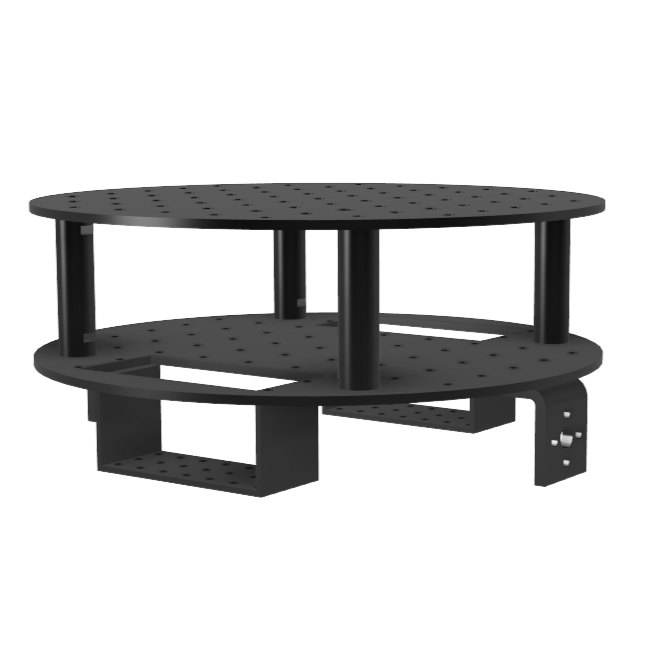
\includegraphics[width=\textwidth]{images/model_top.png}
		\caption{Side view of the robot chassis with both base and top plate visible.}
        \label{fig:top_chassis}
	\end{subfigure}
    \hfill
	\begin{subfigure}[t]{0.49\columnwidth}
		\centering
		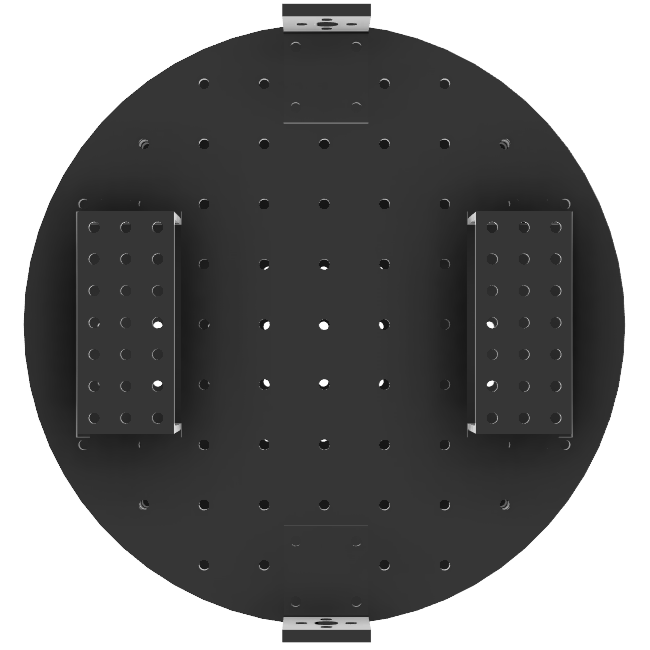
\includegraphics[width=\textwidth]{images/model_bot.png}
		\caption{Bottom view of robot chassis, only base plate visible.}
        \label{fig:bottom_chassis}
	\end{subfigure}
	\caption{The 3D printed robot chassis.}
    \label{fig:robot_chassis}
\end{figure}
% Wiring diagram
A wiring diagram for all the electrical components can be seen in Fig.\:\ref{fig:wiringD}.
\begin{figure}
    \centering
    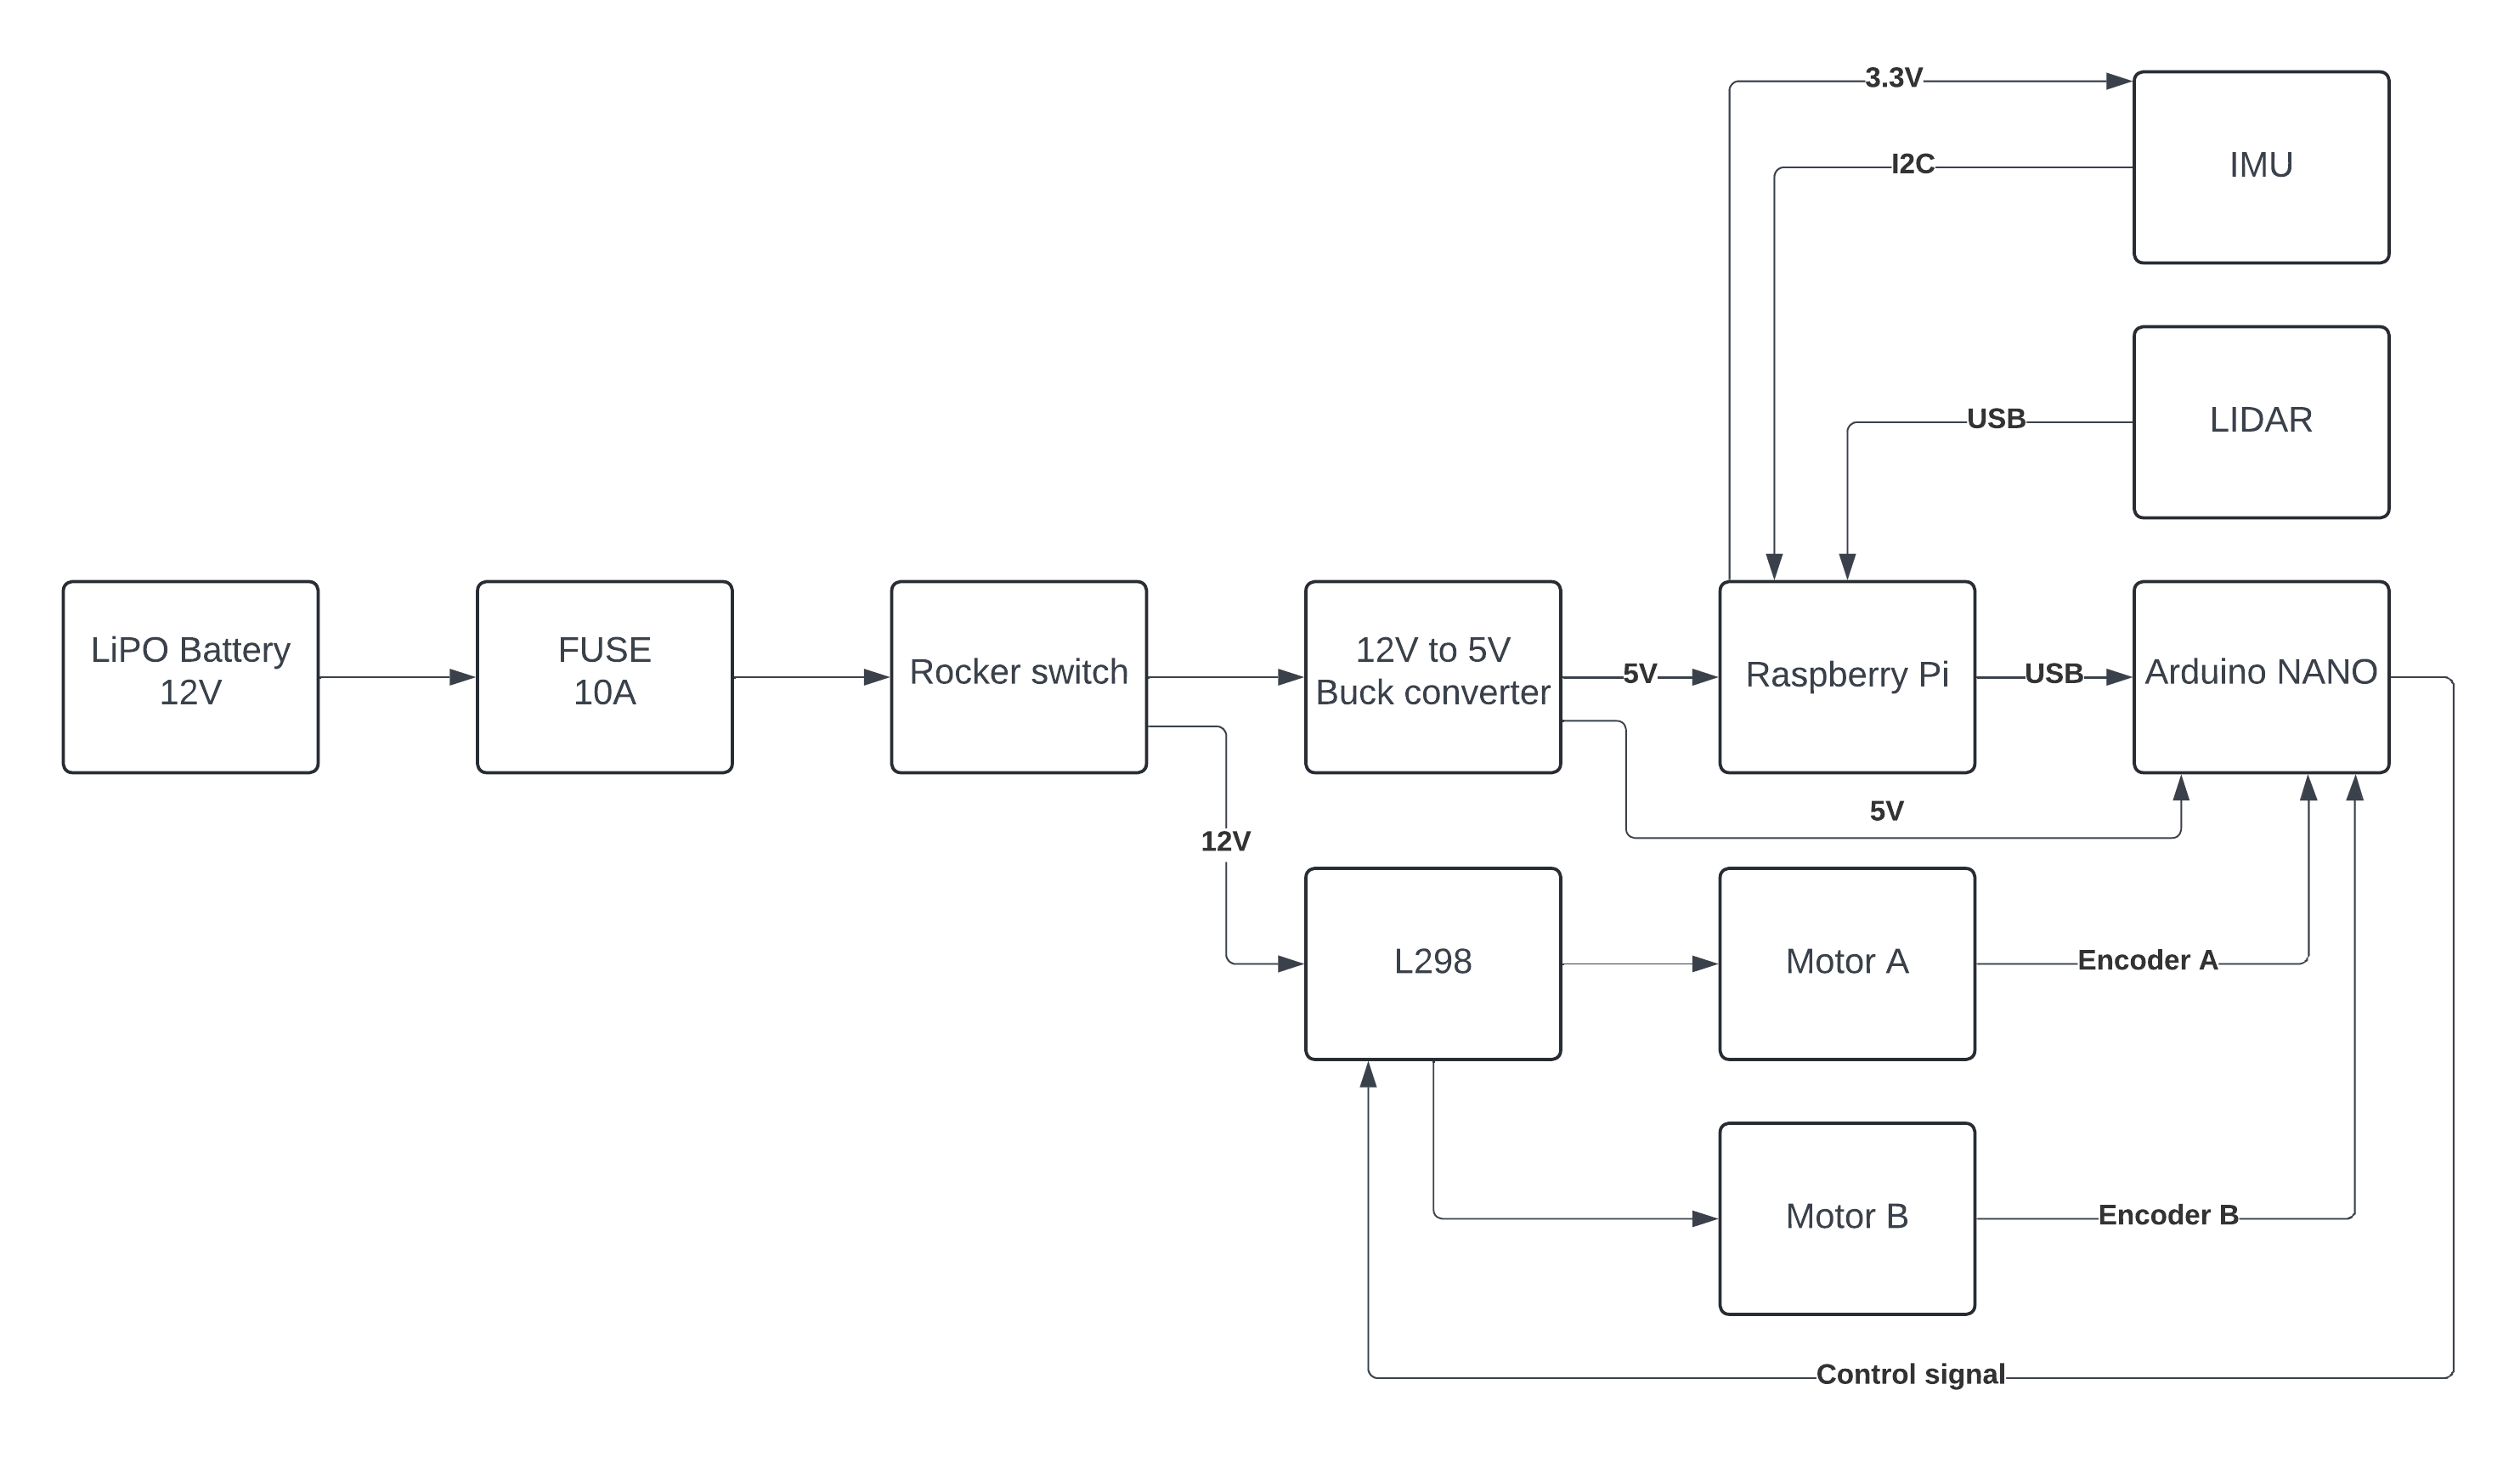
\includegraphics[width=\columnwidth]{images/wiringD.png}
    \caption{Wiring diagram for all electrical components.}
    \label{fig:wiringD}
\end{figure}
% Locations of parts on chassis
The LIDAR and the power source were attached to the top plate of the robot chassis, see Fig.\:\ref{fig:constructed_robot_top_plate}. Mounted on the upper side of the base plate were: the Raspberry Pi, Arduino Nano, IMU, toggle switch, buck converter and fuses, as can be seen in Fig.\:\ref{fig:constructed_robot_top}, with motor driver installed on the bottom side of the base plate, see Fig.\:\ref{fig:constructed_robot_bot}. The motorized wheels were attached to the middle of the base plate, with one spherical wheel attached in the front and one in the back to balance it, see Fig.\:\ref{fig:constructed_robot_bot}. 
% 4 wheel reason
Given that the axle of the motorized wheels runs along the middle of the robot, a single stabilizing wheel proved insufficient, necessitating an additional stabilizing wheel to prevent tipping, especially during acceleration.

% Final real world robot
The finalized robot which was used for real-world testing can be seen in Fig.\:\ref{fig:constructed_robot}.
\begin{figure}
    \centering
    \begin{subfigure}[t]{0.32\columnwidth}
        \centering
        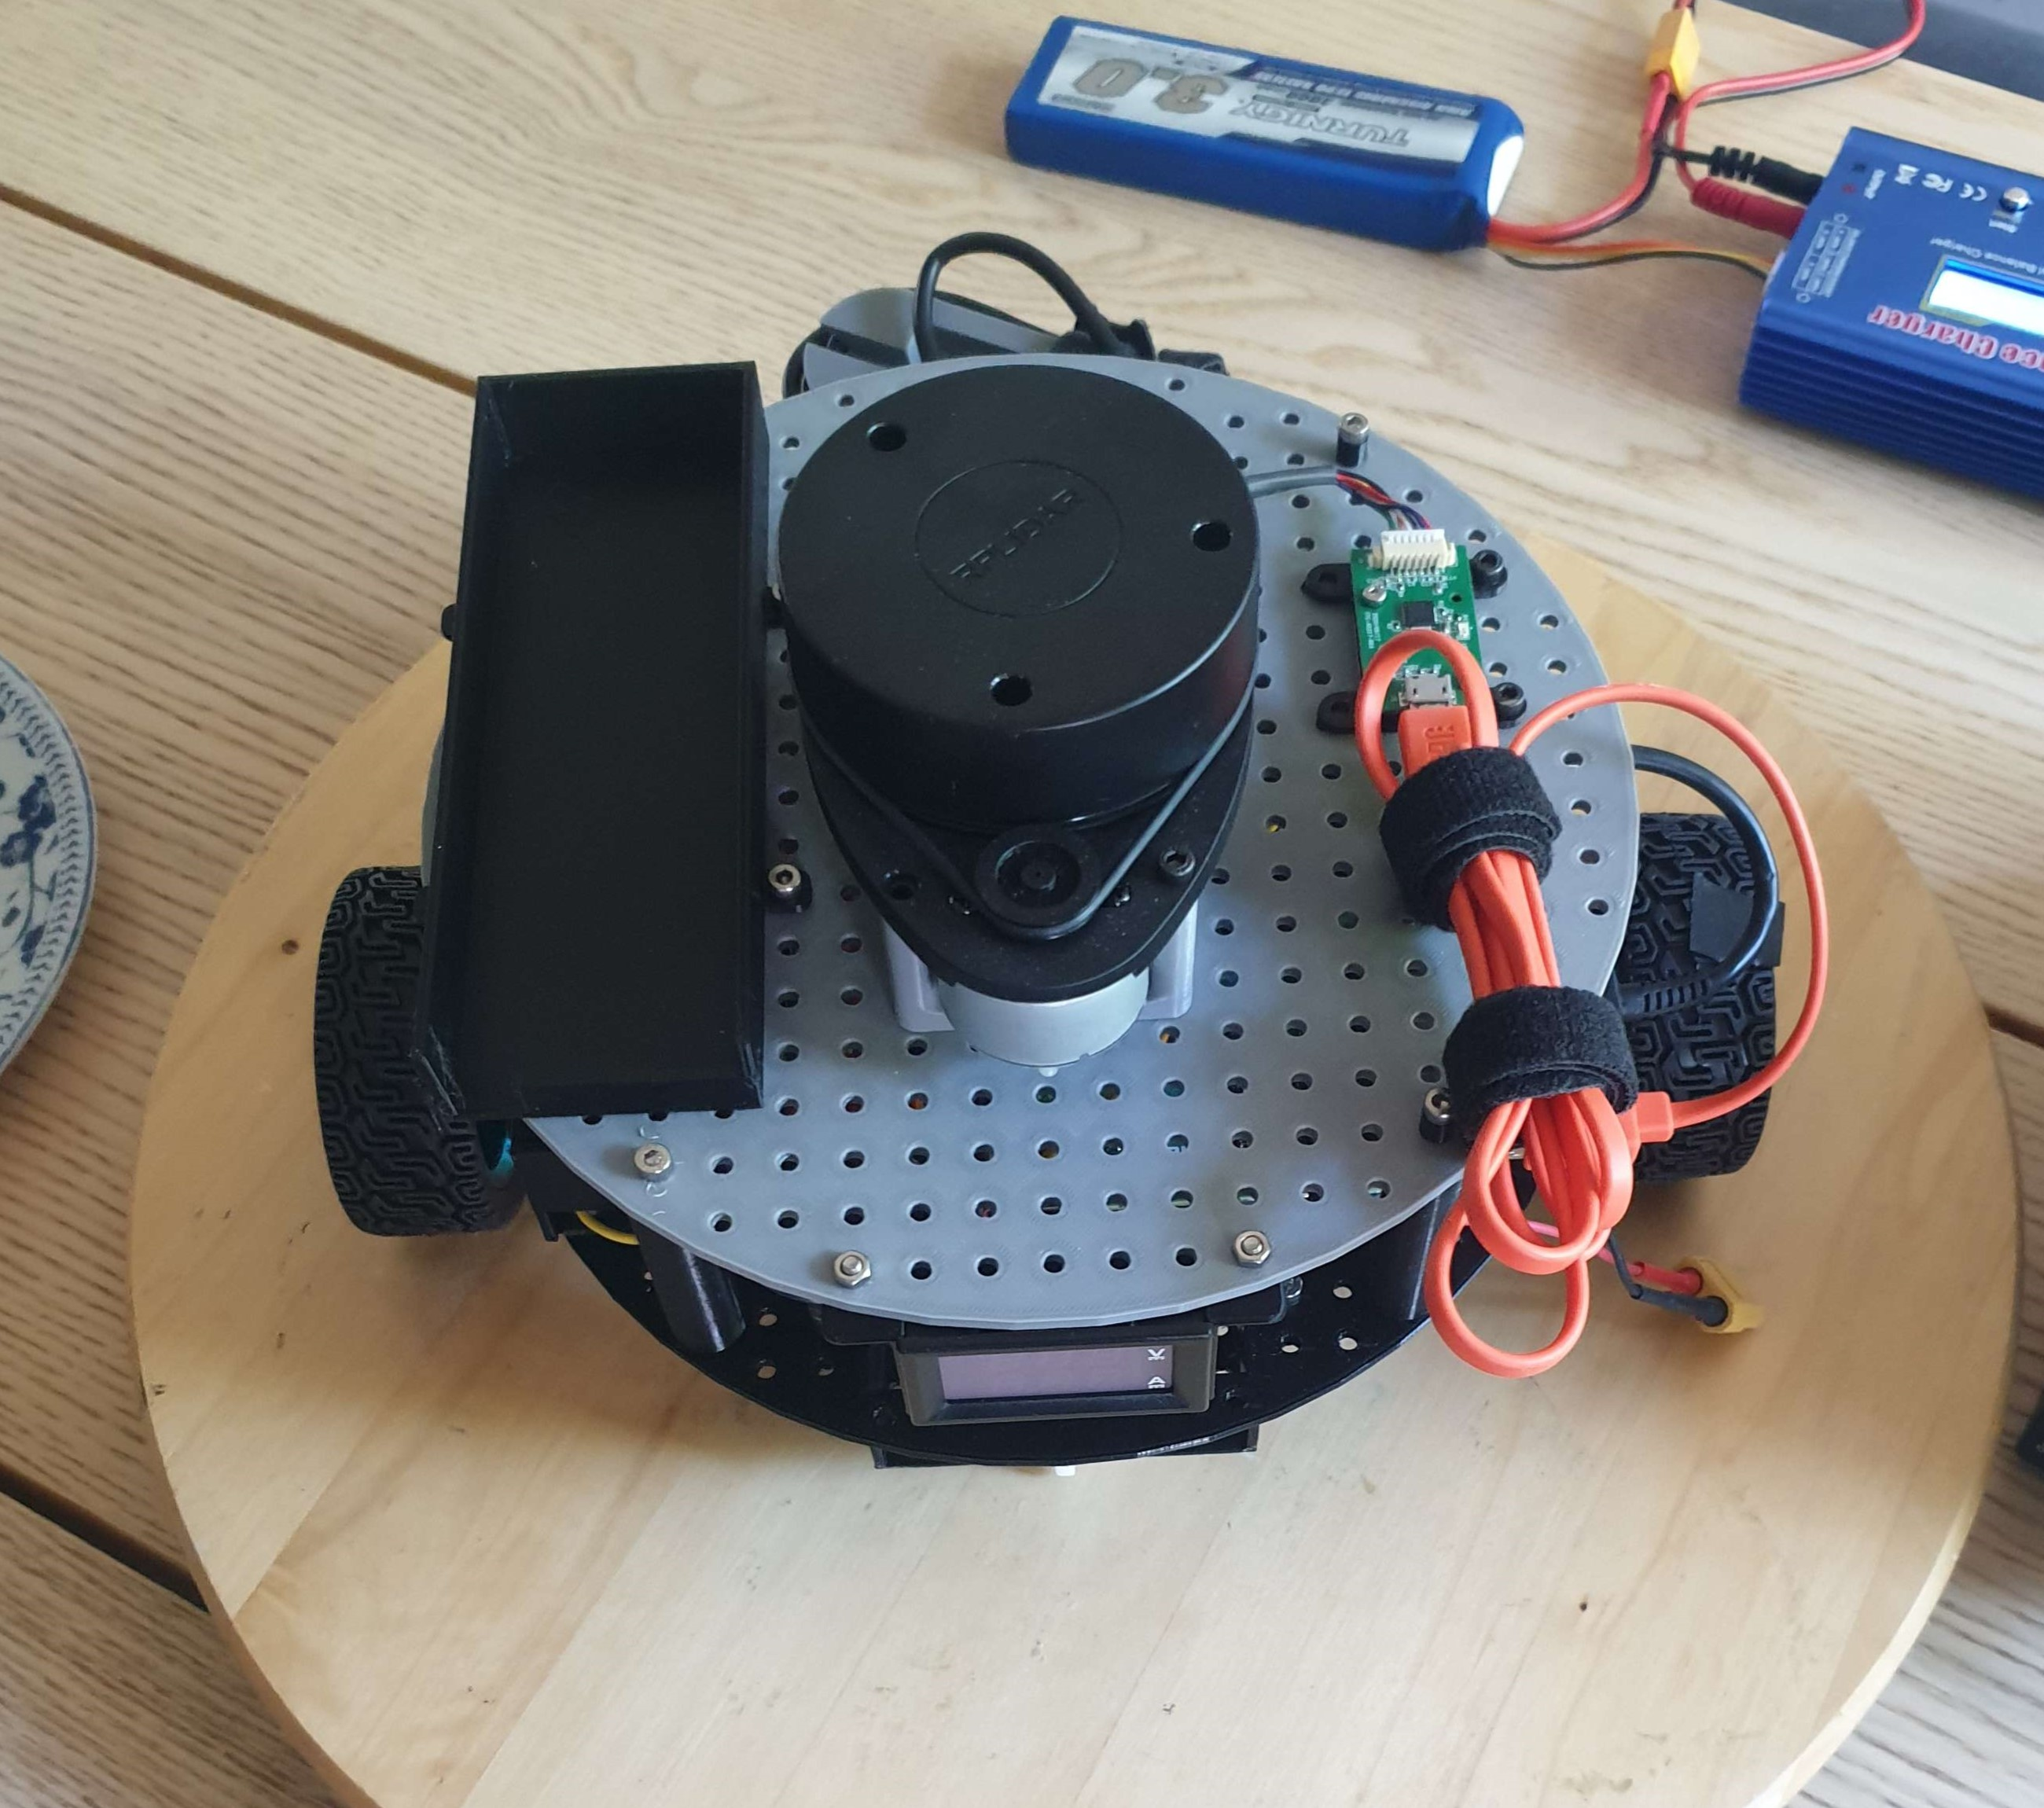
\includegraphics[width=\textwidth]{images/real_robot_top_plate.jpg}
        \caption{Top view of the constructed robot, with top plate attached.}
        \label{fig:constructed_robot_top_plate}
    \end{subfigure}
    \hfill
	\begin{subfigure}[t]{0.32\columnwidth}
		\centering
		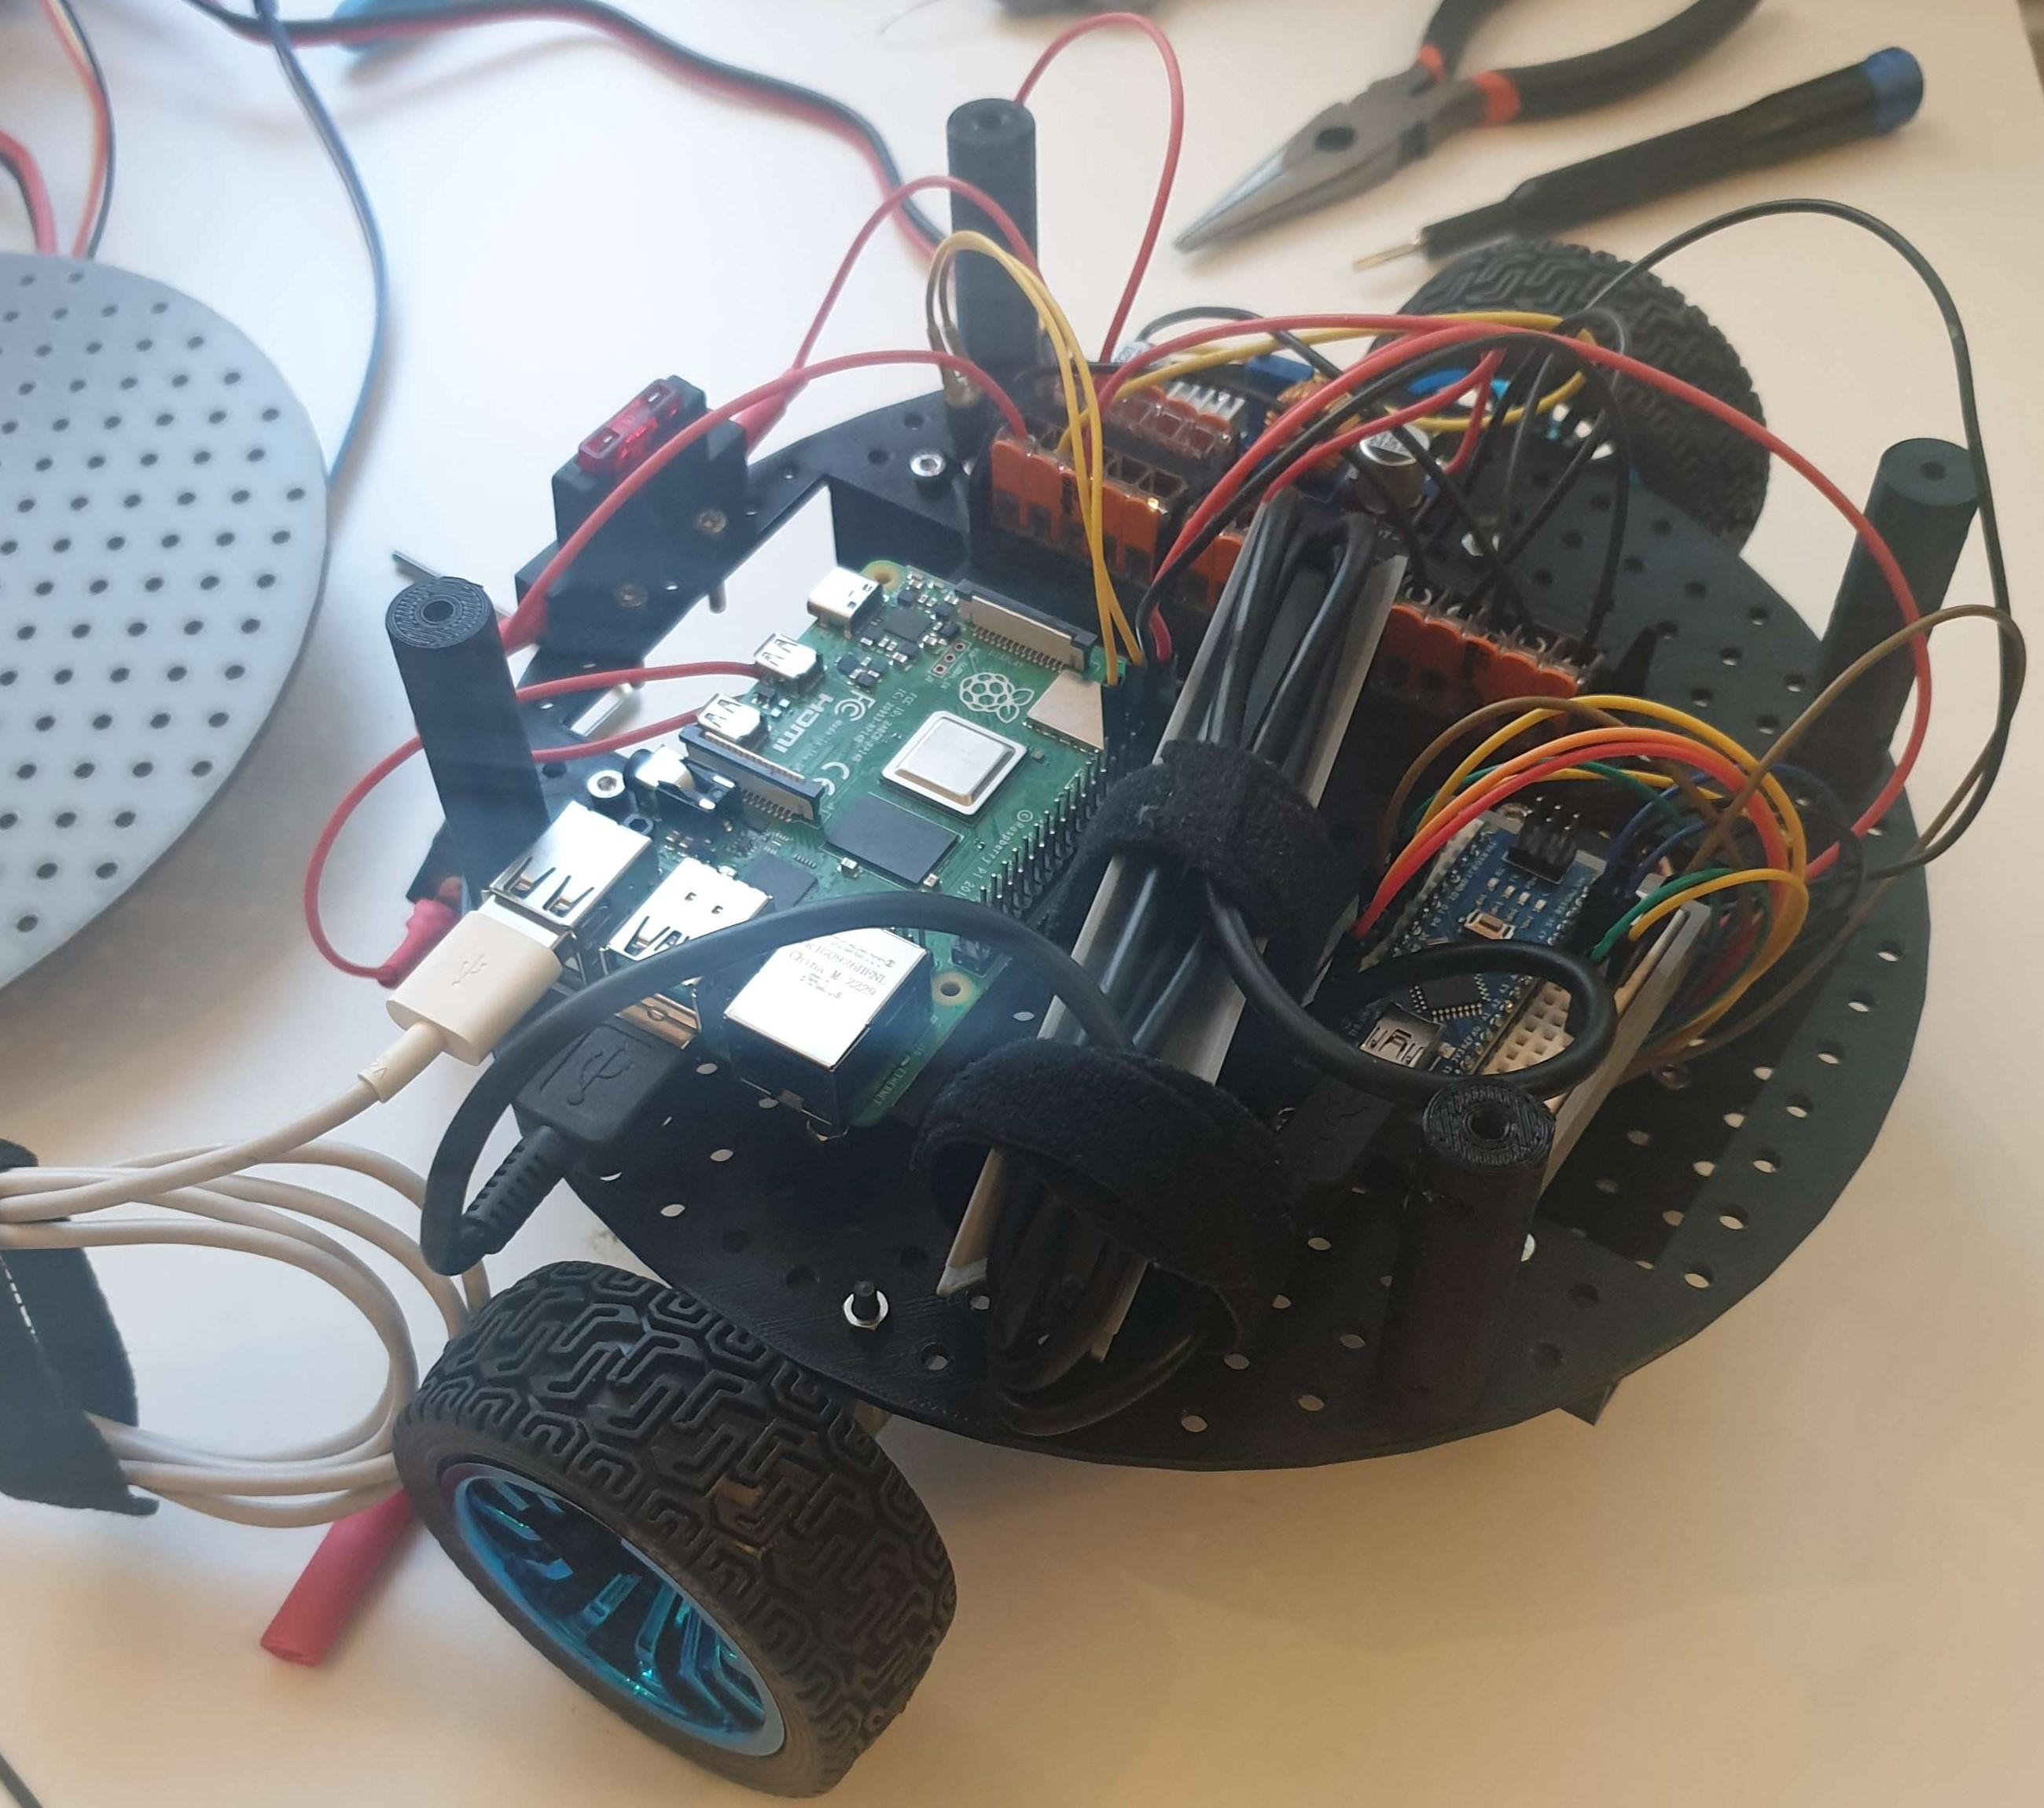
\includegraphics[width=\textwidth]{images/real_robot_top.jpg}
		\caption{Top view of the constructed robot, with top plate removed for clarity of component locations.}
        \label{fig:constructed_robot_top}
	\end{subfigure}
    \hfill
	\begin{subfigure}[t]{0.32\columnwidth}
		\centering
		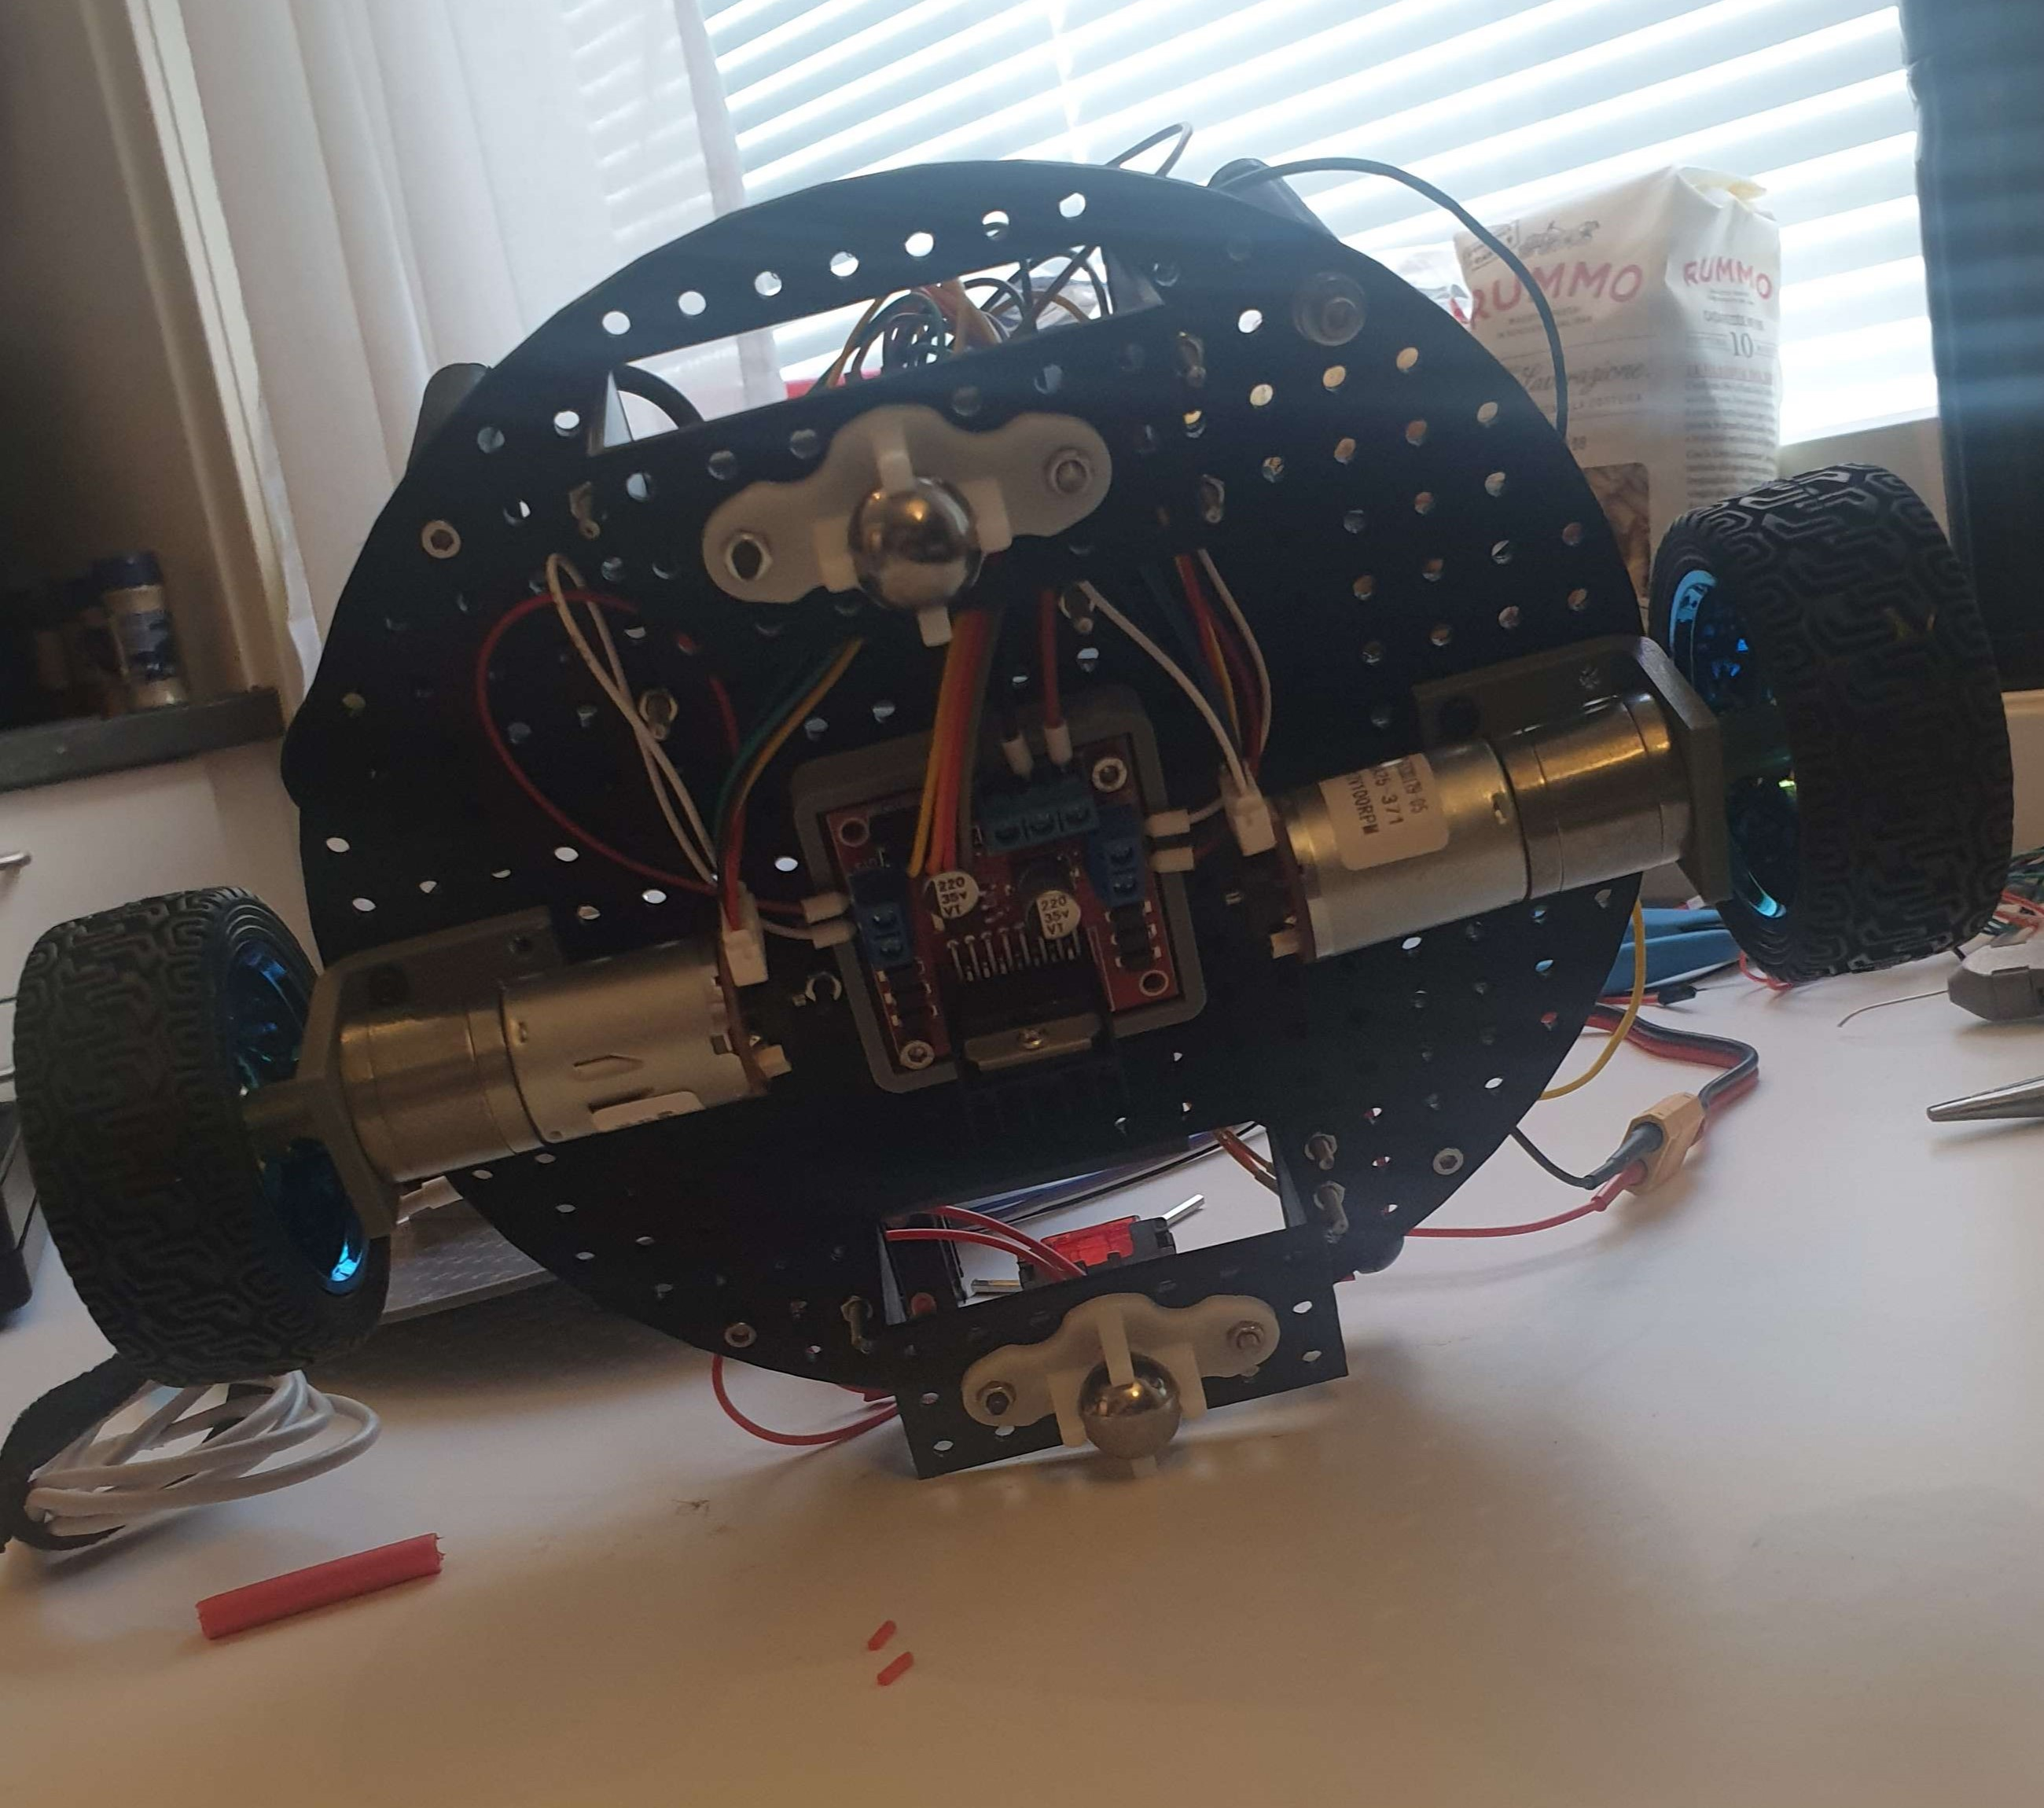
\includegraphics[width=\textwidth]{images/real_robot_bot.jpg}
		\caption{Bottom view of the constructed robot.}
        \label{fig:constructed_robot_bot}
	\end{subfigure}
    \caption{The finalized robot used for real-world testing.}
    \label{fig:constructed_robot}
\end{figure}

%------------------------------------------------------------------------------------------
% Sensors

\subsection{Sensors}

% Purpose
This project used two wheel encoders and a \href{https://www.mouser.se/ProductDetail/426-SEN0142}{6-DOF IMU}, consisting of a 3-DOF MEMS (microelectromechanical system) gyroscope and accelerometer\:\cite{invensense_mpu-6000_2013}, for obtaining odometry information as suggested by the Introduction\:\ref{section:intro}. A \href{https://www.mouser.se/ProductDetail/426-DFR0315}{2D LIDAR} was used for measuring the surrounding, given its compatibility with the toolboxes used and the criteria established, see Introduction\:\ref{section:intro}.

% BAISC FUNCTIONALITY OF SENSORS WHICH ONLY CONCERNS ELA400
% THIS FILE IS ELA400 SPECIFIC, CONTAINING SENSOR FUNCTIONALITY INFORMATION WHICH IS NOT NECESSARY FOR ELA408
%------------------------------------------------------------------------------------------

% !!! LEAVE EMPTY FOR ELA408 REPORT !!!

%------------------------------------------------------------------------------------------

%------------------------------------------------------------------------------------------

% ROS2

\subsection{ROS2}

% Overview
ROS2 contributes to easy development of robotic systems and applications, it offers middleware, algorithms and developer tools\:\cite{macenski_robot_2022}. 
% Purpose
The integration of ROS2 is crucial for easy and quick development as well as its critical purpose in the system. Handling communication, interaction between different parts of the system, and being compatible with the toolboxes used\:\cite{macenski_impact_2023}\cite{macenski_robot_2022}.

% TOOLBOX INFORMATION WHICH ONLY CONCERNS ELA408
% THIS FILE IS ELA408 SPECIFIC, CONTAINING TOOLBOX INFORMATION WHICH IS NOT NECESSARY FOR ELA400
%------------------------------------------------------------------------------------------

% Overview
ROS2 was developed to provide modular and distributed systems, allowing much of the work to be reused and easily adapted to new and similar applications, facilitating collaboration and cooperation\:\cite{macenski_robot_2022}. It has real time capabilities and works on embedded systems as well as in diverse network conditions and environments\:\cite{macenski_robot_2022}.
% Features
% Sensor fusion
Among all of the the features offered by ROS2, one of them is sensor fusion, using either an extended Kalman filter (EKF) or an unscented Kalman filter (UKF)\:\cite{macenski_desks_2023}. 
% Localization
It also offers an AMCL (adaptive Monte Carlo localization) package for localization\:\cite{macenski_desks_2023}. 
% Utility functions
Additionally, ROS2 offers a number of utility functions to improve safety by giving commands, regulating and validating the robotic system and its navigation\:\cite{macenski_desks_2023}. Included in these are collision monitoring which overrides the navigation planner in case of emergencies, and lifecycle manger which ensures that the system starts up and shuts down in a safe and deterministic manner\:\cite{macenski_desks_2023}. 
% More info
For additional information about features offered by ROS2, see\:\cite{macenski_desks_2023}, and for a deeper understanding of ROS2, see\:\cite{macenski_robot_2022}.

%------------------------------------------------------------------------------------------


%------------------------------------------------------------------------------------------
\begin{comment}
    
\end{comment}
%------------------------------------------------------------------------------------------

% Default and changed parameters
The ROS2 parameters which were changed from their default value are shown in Fig.\:\ref{tab:ros2_params_changed}, parameters which are not listed had their default value.
\begin{table}
    \centering
    \begin{tabular}{|c|c|} \hline
         \textbf{Parameter}         & \textbf{Value}    \\ \hline
         Sensor fusion              & EKF               \\ \hline
    \end{tabular}
    \caption{ROS2 parameters which were changed from their default value.}
    \label{tab:ros2_params_changed}
\end{table}
EKF was used for sensor fusion since it provided the best results.

%------------------------------------------------------------------------------------------
% SLAM

\subsection{SLAM Toolbox}

% Purpose
The SLAM tool used in this project is an open source toolbox called SLAM Toolbox, which is built on top of OpenKarto SLAM\:\cite{macenski_slam_2021}\cite{macenski_desks_2023}\cite{macenski_use_2019}.
% World model
SLAM Toolbox uses elastic pose-graph representation for localization and mapping\:\cite{macenski_use_2019}, which can be converted to a 2D probabilistic occupancy grid map\:\cite{macenski_slam_2021}. 
% Scan matching, loop closure, link matching, scan correlation
It offers scan matching (which uses a correlation grid), loop closing, link matching algorithm and scan correlation\:\cite{macenski_slam_2021}.

% TOOLBOX INFORMATION WHICH ONLY CONCERNS ELA408
% THIS FILE IS ELA408 SPECIFIC, CONTAINING TOOLBOX INFORMATION WHICH IS NOT NECESSARY FOR ELA400
%------------------------------------------------------------------------------------------

% Boasted features
SLAM Toolbox boasts a number of impressive features compared to its competitors, including\:\cite{macenski_slam_2021}:
\begin{itemize}
    \item Being able to map areas as large as $9000\:\text{m}^2$
    \item Serialize (save) and deserialize (load) map, allowing for continued expanding of a previous map
    \item Being able to merge multiple maps using kinematic map merging
    \item Being able to perform synchronous mapping, asynchronous mapping or pure localization
    \item Faster measurement matching, better optimization and more (see\:\cite{macenski_slam_2021})
\end{itemize}
% Lifelong mapping
It offers has a functionality called lifelong mapping which not only allows SLAM to continue refining the map and update it, but also remove redundant and outdated data by the help of a heuristic\:\cite{macenski_use_2019}. 
% KD-Tree
On top of that it also makes use of k-dimensional trees (KD-Tree) to perform search matching (nearest neighbor search matching) for localization of the robot position\:\cite{macenski_slam_2021}.
% Parameters etc
A subset of the parameter options offered by SLAM Toolbox are outlined in Table.\:\ref{tab:slam_toolbox_params}\:\cite{macenski_slam_2021}\cite{macenski_use_2019}.
\begin{table}
    \centering
    \resizebox{\columnwidth}{!}{\noindent\begin{tabular}{|c|c|} \hline
         \textbf{Parameter}                                         & \textbf{Options}                                      \\ \hline
         Nonlinear solver                                           & Ceres solver                                          \\
                                                                    & SPA solver                                            \\
                                                                    & g2o solver                                            \\ \hline
         Linear solver used by Ceres                                & sparse Cholesky factorization                         \\
                                                                    & Schur complement                                      \\
                                                                    & Schur complement and iterative solver                 \\
                                                                    & CGNR (conjugate gradient normal residual)             \\ \hline
         Preconditioner  to use with linear solver                  & Identity (none)                                       \\
                                                                    & Jacobi                                                \\
                                                                    & Schur complement Jacobi                               \\ \hline
         Ceres trust region strategy                                & Levenberg-Marquardt algorithm                         \\
                                                                    & Dogleg algorithm                                      \\ \hline
         Dogleg strategy to use if the trust strategy is Dogleg     & Traditional Dogleg                                    \\
                                                                    & Subspace Dogleg                                       \\ \hline
         Loss function to reject outliers                           & None                                                  \\
                                                                    & Huber loss                                            \\
                                                                    & Cauchy loss                                           \\ \hline
        KD-Tree distance metric                                     & Manhattan distance functor                            \\ 
                                                                    & Squared Euclidean distance functor                    \\
                                                                    & Squared Euclidean (L2) distance functor               \\
                                                                    & SO2 distance functor                                  \\
                                                                    & SO3 distance functor (uses L2\_Simple)                \\ \hline
    \end{tabular}}
    \caption{A subset of the parameter options offered by SLAM Toolbox\:\cite{macenski_slam_2021}\cite{macenski_use_2019}.}
    \label{tab:slam_toolbox_params}
\end{table}

%------------------------------------------------------------------------------------------


%------------------------------------------------------------------------------------------
\begin{comment}
    %The occupancy grid map has default scale of $1\:\text{grid coordinate} = 1\:\text{pixel} = 0.05\:\text{meters}$\:\cite{macenski_slam_2021}\cite{macenski_use_2019}.    
\end{comment}
%------------------------------------------------------------------------------------------

% Default and changed parameters
The default parameters of SLAM Toolbox has been shown to perform the best in normal situations\:\cite{macenski_slam_2021}\cite{macenski_use_2019}, minimal alterations were therefor attempted. All parameters which were changed from their default value are shown in Table.\:\ref{tab:slam_toolbox_params_changed}.
\begin{table}
    \centering
    \begin{tabular}{|c|c|} \hline
         \textbf{Parameter}         & \textbf{Value}    \\ \hline
         Laser\_range               & 6.0               \\ \hline
         Barycentering              & False             \\ \hline
         map\_update\_interval      & 1.0               \\ \hline
         scan\_buffer\_size         & 100               \\ \hline
         stack\_size\_to\_use       & 90000000          \\ \hline
    \end{tabular}
    \caption{SLAM Toolbox parameters which were changed from their default.}
    \label{tab:slam_toolbox_params_changed}
\end{table}
Laser\_range was changed because of the LIDAR used. Barycentering was set to False and scan pose was thus used instead of barycentering since it made the mapping more accurate. The remaining parameters were found during testing to provide the best performance.

% SLAM Toolbox Flowchart
The complete functionality of SLAM Toolbox can be seen in Fig.\:\ref{fig:slam_toolbox}.
\begin{figure*}
    \centering
    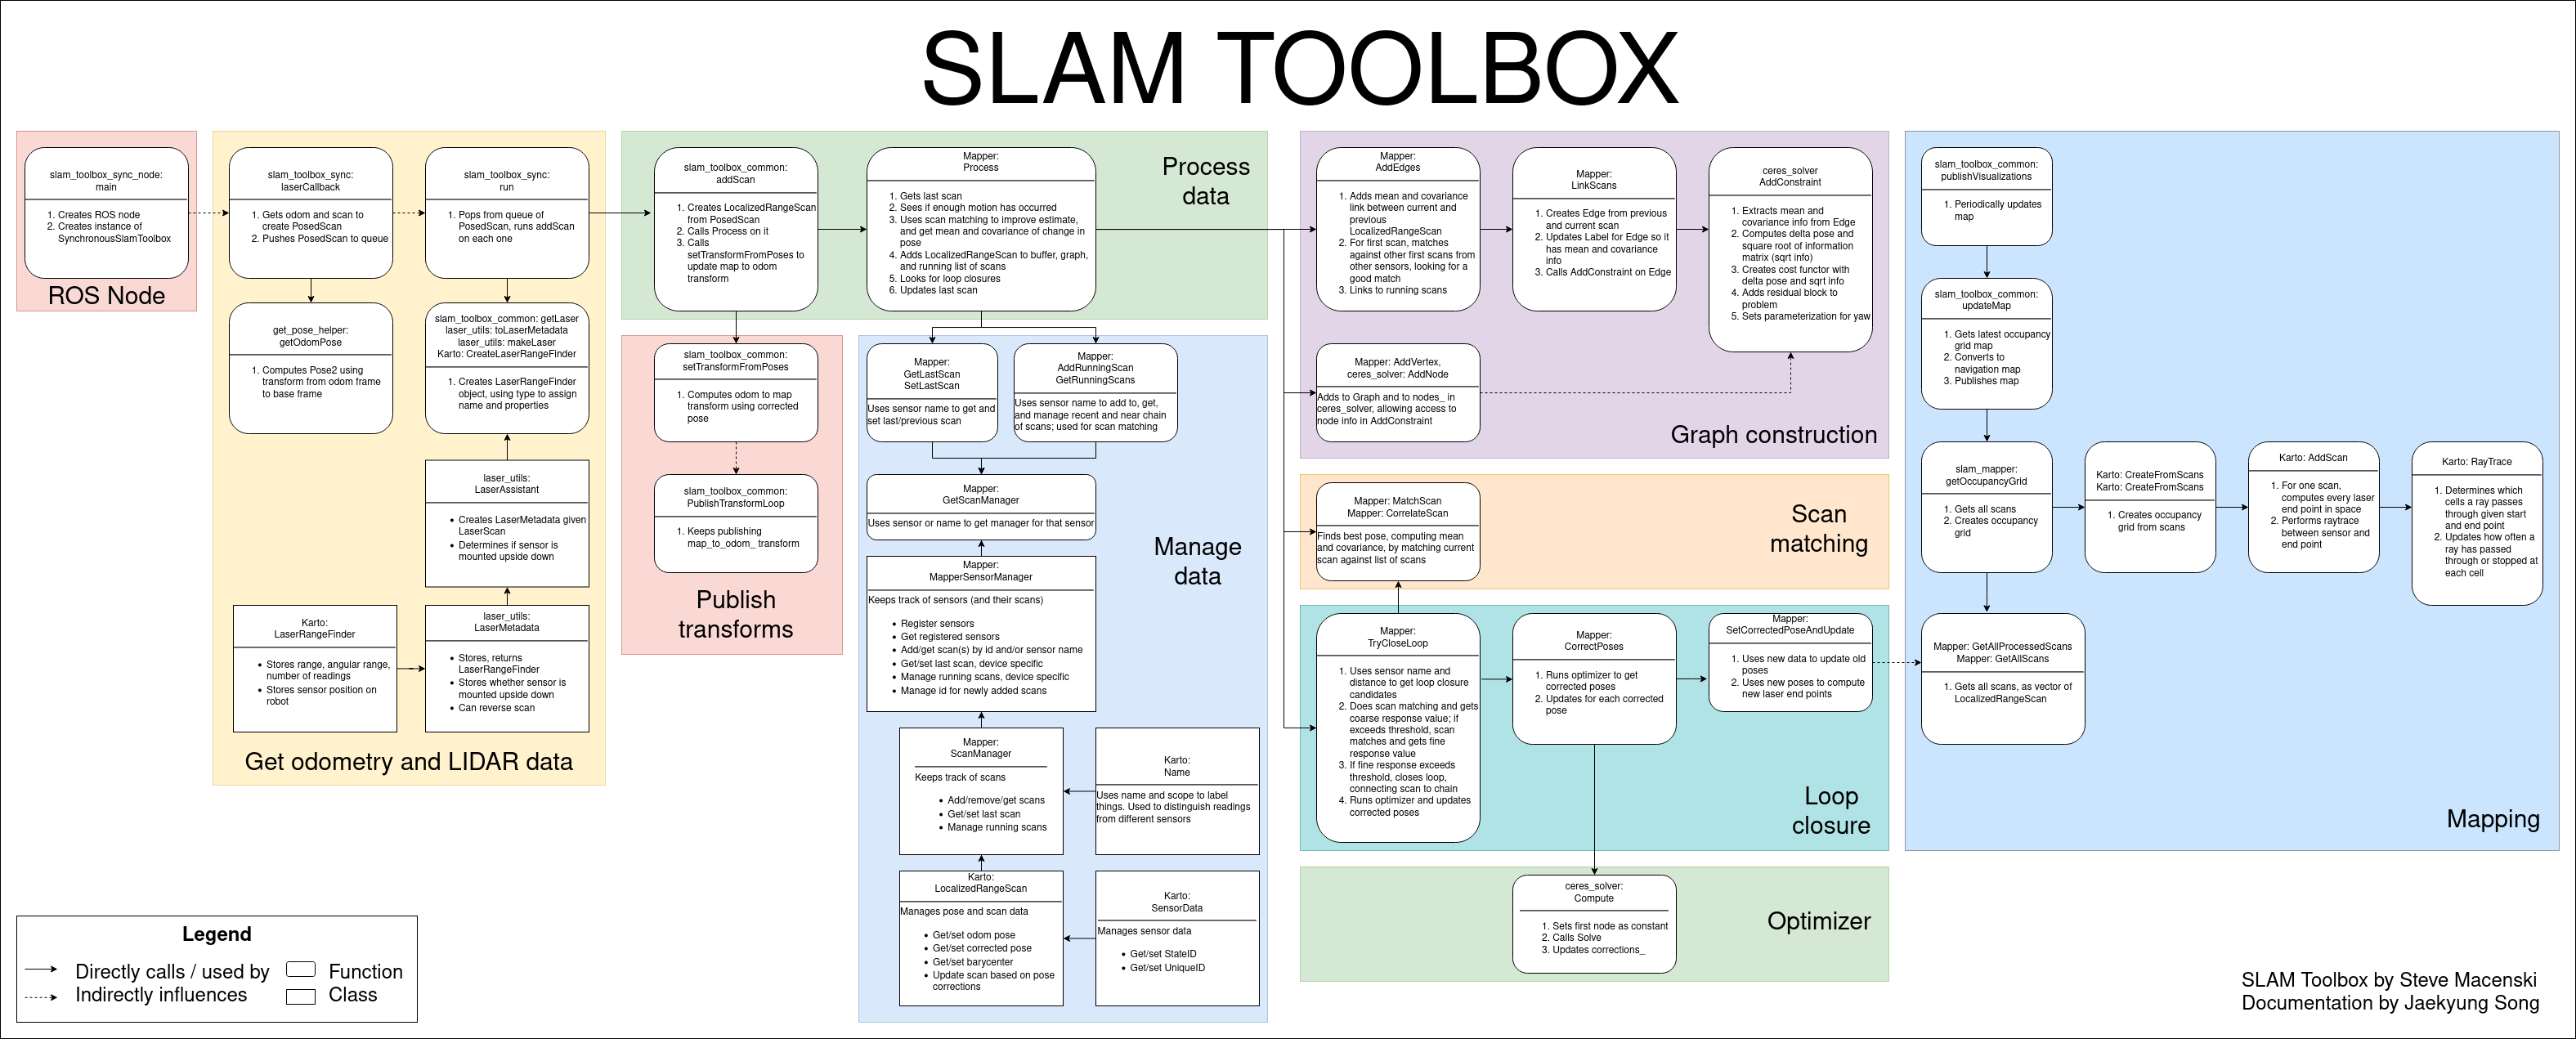
\includegraphics[width=\textwidth]{images/slam_toolbox_sync.png}
    \caption{SLAM Toolbox flowchart showing the functionality of the toolbox. Courtesy of Steven Macenski (creator)\:\cite{macenski_slam_2021}\cite{macenski_use_2019}.}
    \label{fig:slam_toolbox}
\end{figure*}

%------------------------------------------------------------------------------------------
% Navigation

\subsection{Navigation2}

% Purpose
This project used the optimized open source toolbox Navigation2 (Nav2), for proficient robot navigation and path planning\:\cite{macenski_desks_2023}\cite{macenski_open-source_2024}\cite{macenski_regulated_2023}\cite{merzlyakov_comparison_2021}\cite{macenski_marathon_2020}.
% Global, local and recovery
Nav2 performs three tasks: planning (global path planning), control (local trajectory tracking) and recovery, orchestrated by a configurable behavior tree\:\cite{macenski_marathon_2020}. The three tasks are nodes in the behavior tree with the navigator as the root, all of them sharing a costmap model of the environment\:\cite{macenski_marathon_2020}.

% TOOLBOX INFORMATION WHICH ONLY CONCERNS ELA408
% THIS FILE IS ELA408 SPECIFIC, CONTAINING TOOLBOX INFORMATION WHICH IS NOT NECESSARY FOR ELA400
%------------------------------------------------------------------------------------------

% Outline
The design of Nav2 makes it very configurable and expandable, it also works for a multitude of robot types in a wide range of applications and environments\:\cite{macenski_marathon_2020}. It has also been shown to be safe, deterministic, reliable and robust in dynamic settings even during extended time frames\:\cite{macenski_marathon_2020}. 

% Global path planning
% Smac planner (templated A*)
Smac planner is the standard global path planning system used by Nav2\:\cite{macenski_open-source_2024}. It uses a templated A* which performs search, and it is templated by node planner templates NodeT which implements the different planner-specifics\:\cite{macenski_open-source_2024}. With this, NodeT can select different templates which results in different planners and characteristics\:\cite{macenski_open-source_2024}. All the planners thus share the same A* algorithm but the cost function and neighborhood selection policies are decoupled\:\cite{macenski_open-source_2024}. This is further clarified when inspecting the node planners which contain two things\:\cite{macenski_open-source_2024}:
\begin{itemize}
    \item Node state: which includes things like collision state, visited status, queued status and accumulated cost of the node in the graph
    \item Planner-specific: which includes how traversal costs should be computed, heuristics and expansion characteristics
\end{itemize}
Three different planner templates (NodeT) are offered, these are: cost-aware 2D-A*, cost-aware Hybrid-A* and cost-aware State Lattice\:\cite{macenski_open-source_2024}. Cost-aware means that additional information is encoded in the map and used by the path planner rather than just the common binary info of occupied or free (see costmap in Introduction\:\ref{section:intro})\:\cite{macenski_open-source_2024}.
Finally there is an integration layer which, on the highest level, links the planner with the robot, thus allowing for easy deployment on multiple robotic frameworks\:\cite{macenski_open-source_2024}.
% Smoothing global paths
Nav2 includes three smoothing algorithms to help refine paths produced by the global path planner, these are: Simple Smoother, Constrained Smoother, and Savitzky-Golay Smoother\:\cite{macenski_desks_2023}.
% Additional info
For the complete specifications of Smac planner, see the work by Macenski \textit{et al.}\:\cite{macenski_open-source_2024}.

% Local path planning
% DWB
The default local trajectory tracker used by Navigation2 is DWB, which is an expansion of Dynamic Window Approach (DWA)\:\cite{liu_path_2023}\cite{macenski_desks_2023}. DWB gathers a set of candidate commands, based on its current velocity and dynamic limits, by sub-sampling feasible velocities from a dynamic window, these velocities are projected forward to generate circular arcs (trajectories)\:\cite{macenski_desks_2023}. These arcs are then evaluated using a set of critic functions (which can optimize for different behaviors), and the best is chosen\:\cite{macenski_desks_2023}.
% Additional info
The interested reader is refereed to\:\cite{macenski_desks_2023} for additional information about the local trajectory tracking offered by Nav2.

% Recovery
Recovery behavior is used to prevent complete navigation failure and follows a protocol where initially the actions are conservative and then become more aggressive\:\cite{macenski_marathon_2020}. The actions can be system wide or specific to a certain task like planning and control\:\cite{macenski_marathon_2020}. Example actions include: clearing costmap, waiting and spinning\:\cite{macenski_marathon_2020}.

%------------------------------------------------------------------------------------------


%------------------------------------------------------------------------------------------
\begin{comment}
    , replacing Navigation Function (NavFn)\:\cite{macenski_desks_2023}
    % RPP
    %A local trajectory planner (path tracking) available in Navigation2 is the Regulated Pure Pursuit algorithm (RPP) which is an extension of Adaptive Pure Pursuit (APP)\:\cite{macenski_regulated_2023}. Compared to normal pure pursuit, this variant uses adaptive lookahead distance and takes into account and adapts linear and angular velocity to increase safety and operability, specifically in constrained and partially observable environments\:\cite{macenski_regulated_2023}. It achieves this by incorporating preemptive collision detection, using regulation heuristics and penalizing being close to obstacles as well as taking sharp turns\:\cite{macenski_regulated_2023}. RPP also achieves better efficiency, and thanks to the higher safety it offers, it allows the system to have higher maximum speed while still remaining safe\:\cite{macenski_regulated_2023}.
    % Additional info
    %For a complete understanding of the RPP algorithm see\:\cite{macenski_regulated_2023}.
\end{comment}
%------------------------------------------------------------------------------------------

% Default and changed parameters
All Navigation2 parameters which were altered in this project can be seen in Table.\:\ref{tab:nav2_params_changed}.
\begin{table}
    \centering
    \begin{tabular}{|c|c|} \hline
         \textbf{Parameter}         & \textbf{Value}        \\ \hline
         odom\_topic                & /odometry/filtered    \\ \hline
    \end{tabular}
    \caption{Navigation2 parameters which were changed from their default.}
    \label{tab:nav2_params_changed}
\end{table}
The odometry used by Navigation2 was changed to the EKF filtered topic which contains the fused joint states of the wheels and the IMU values, provided by ROS2.

%------------------------------------------------------------------------------------------
% Simulation

\subsection{Simulation}
\label{subsection:simulation}

% Integration (how our system works)
During the simulation, all ROS2 nodes were running on a PC. The simulated robot published data-points from the LIDAR, IMU and the joint states of the wheels to their respective topics. The SLAM Toolbox node was subscribed to the LIDAR topic and created the map using the LIDAR values. The map was published to a topic which the Nav2 node was subscribed to. Nav2 then used the map to calculate a path for the robot. Odometry information was also required by the Nav2 node, which was obtained by subscribing to the topic where the EKF published the fused IMU values and wheel positions. The ROS2 node (ros2-control) was then used to control the wheels, based on Nav2 input. To make the robot navigate using Nav2 a target position (waypoint) was marked in Rviz2 (part of ROS2). 

% Simulation tool and test environment (features)
All simulation was done in Gazebo and the test environment can be seen in Fig.\:\ref{fig:simulation_map}. The test environment was static, well lit and cluttered. 
% Test scenario
The simulation testing scenario consisted of a mapping session where the robot mapped the entire testing environment.
% Evaluation metrics
The metrics used to evaluate the simulated system were as follows: 
\begin{itemize}
    \item SLAM map compared to ground truth map
    \item Number of collisions
    \item Processing time per sensor update (ms)
\end{itemize}

\begin{figure}
    \centering
    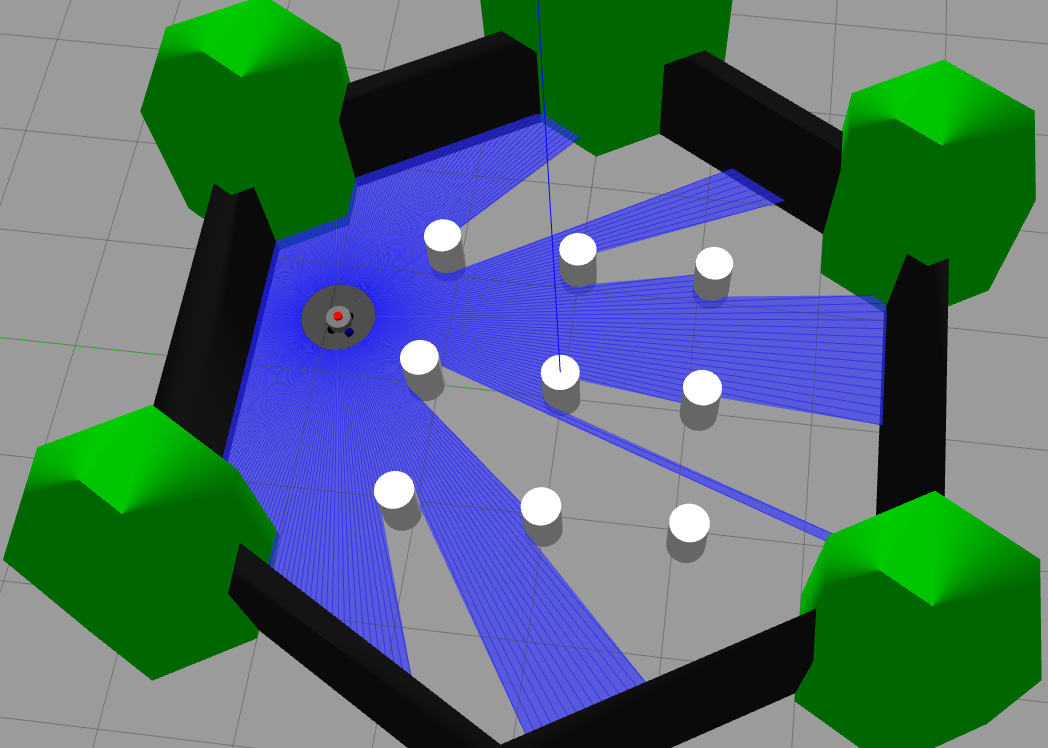
\includegraphics[width=\columnwidth]{images/simulation_map.png}
    \caption{Simulation test environment, also showing the simulated robot.}
    \label{fig:simulation_map}
\end{figure}

%------------------------------------------------------------------------------------------
% Real world

\subsection{Real-world}
\label{subsection:real_world}

% Integration (how our system works)
Four ROS2 nodes were running on the robot (Raspberry Pi), these are the robot-state-publisher, rplidar, mpu6050 and ros2-control. The robot-state-publisher publishes the joint state values for the wheels, the mpu6050 publishes the IMU sensor values and rplidar publishes the LIDAR sensor values.
Finally, the ros2-control node takes the desired input velocity and communicates this through a hardware interface to the Arduino Nano which in turn controls the wheels.
The SLAM Toolbox, Nav2 and EKF filtering nodes were running on an external PC and works the same as in the simulation, issuing of waypoints also works the same as in simulation (see Method\:\ref{subsection:simulation}).

% Test environment (features)
The robot was deployed in an apartment which served as the real-world test environment and can be seen in Fig.\:\ref{fig:real_world_map}. The test environment thus consisted of a static indoor environment which had constant lighting and was open. 
% Test scenario
The real-world testing scenario involved a mapping session where the robot mapped the entire testing environment.
% Evaluation metrics
The real-world deployment of the system was evaluated in terms of the following metrics:
\begin{itemize}
    \item SLAM map compared to ground truth map
    \item Number of collisions
    \item Processing time per sensor update (ms)
\end{itemize}

\begin{figure}
    \centering
    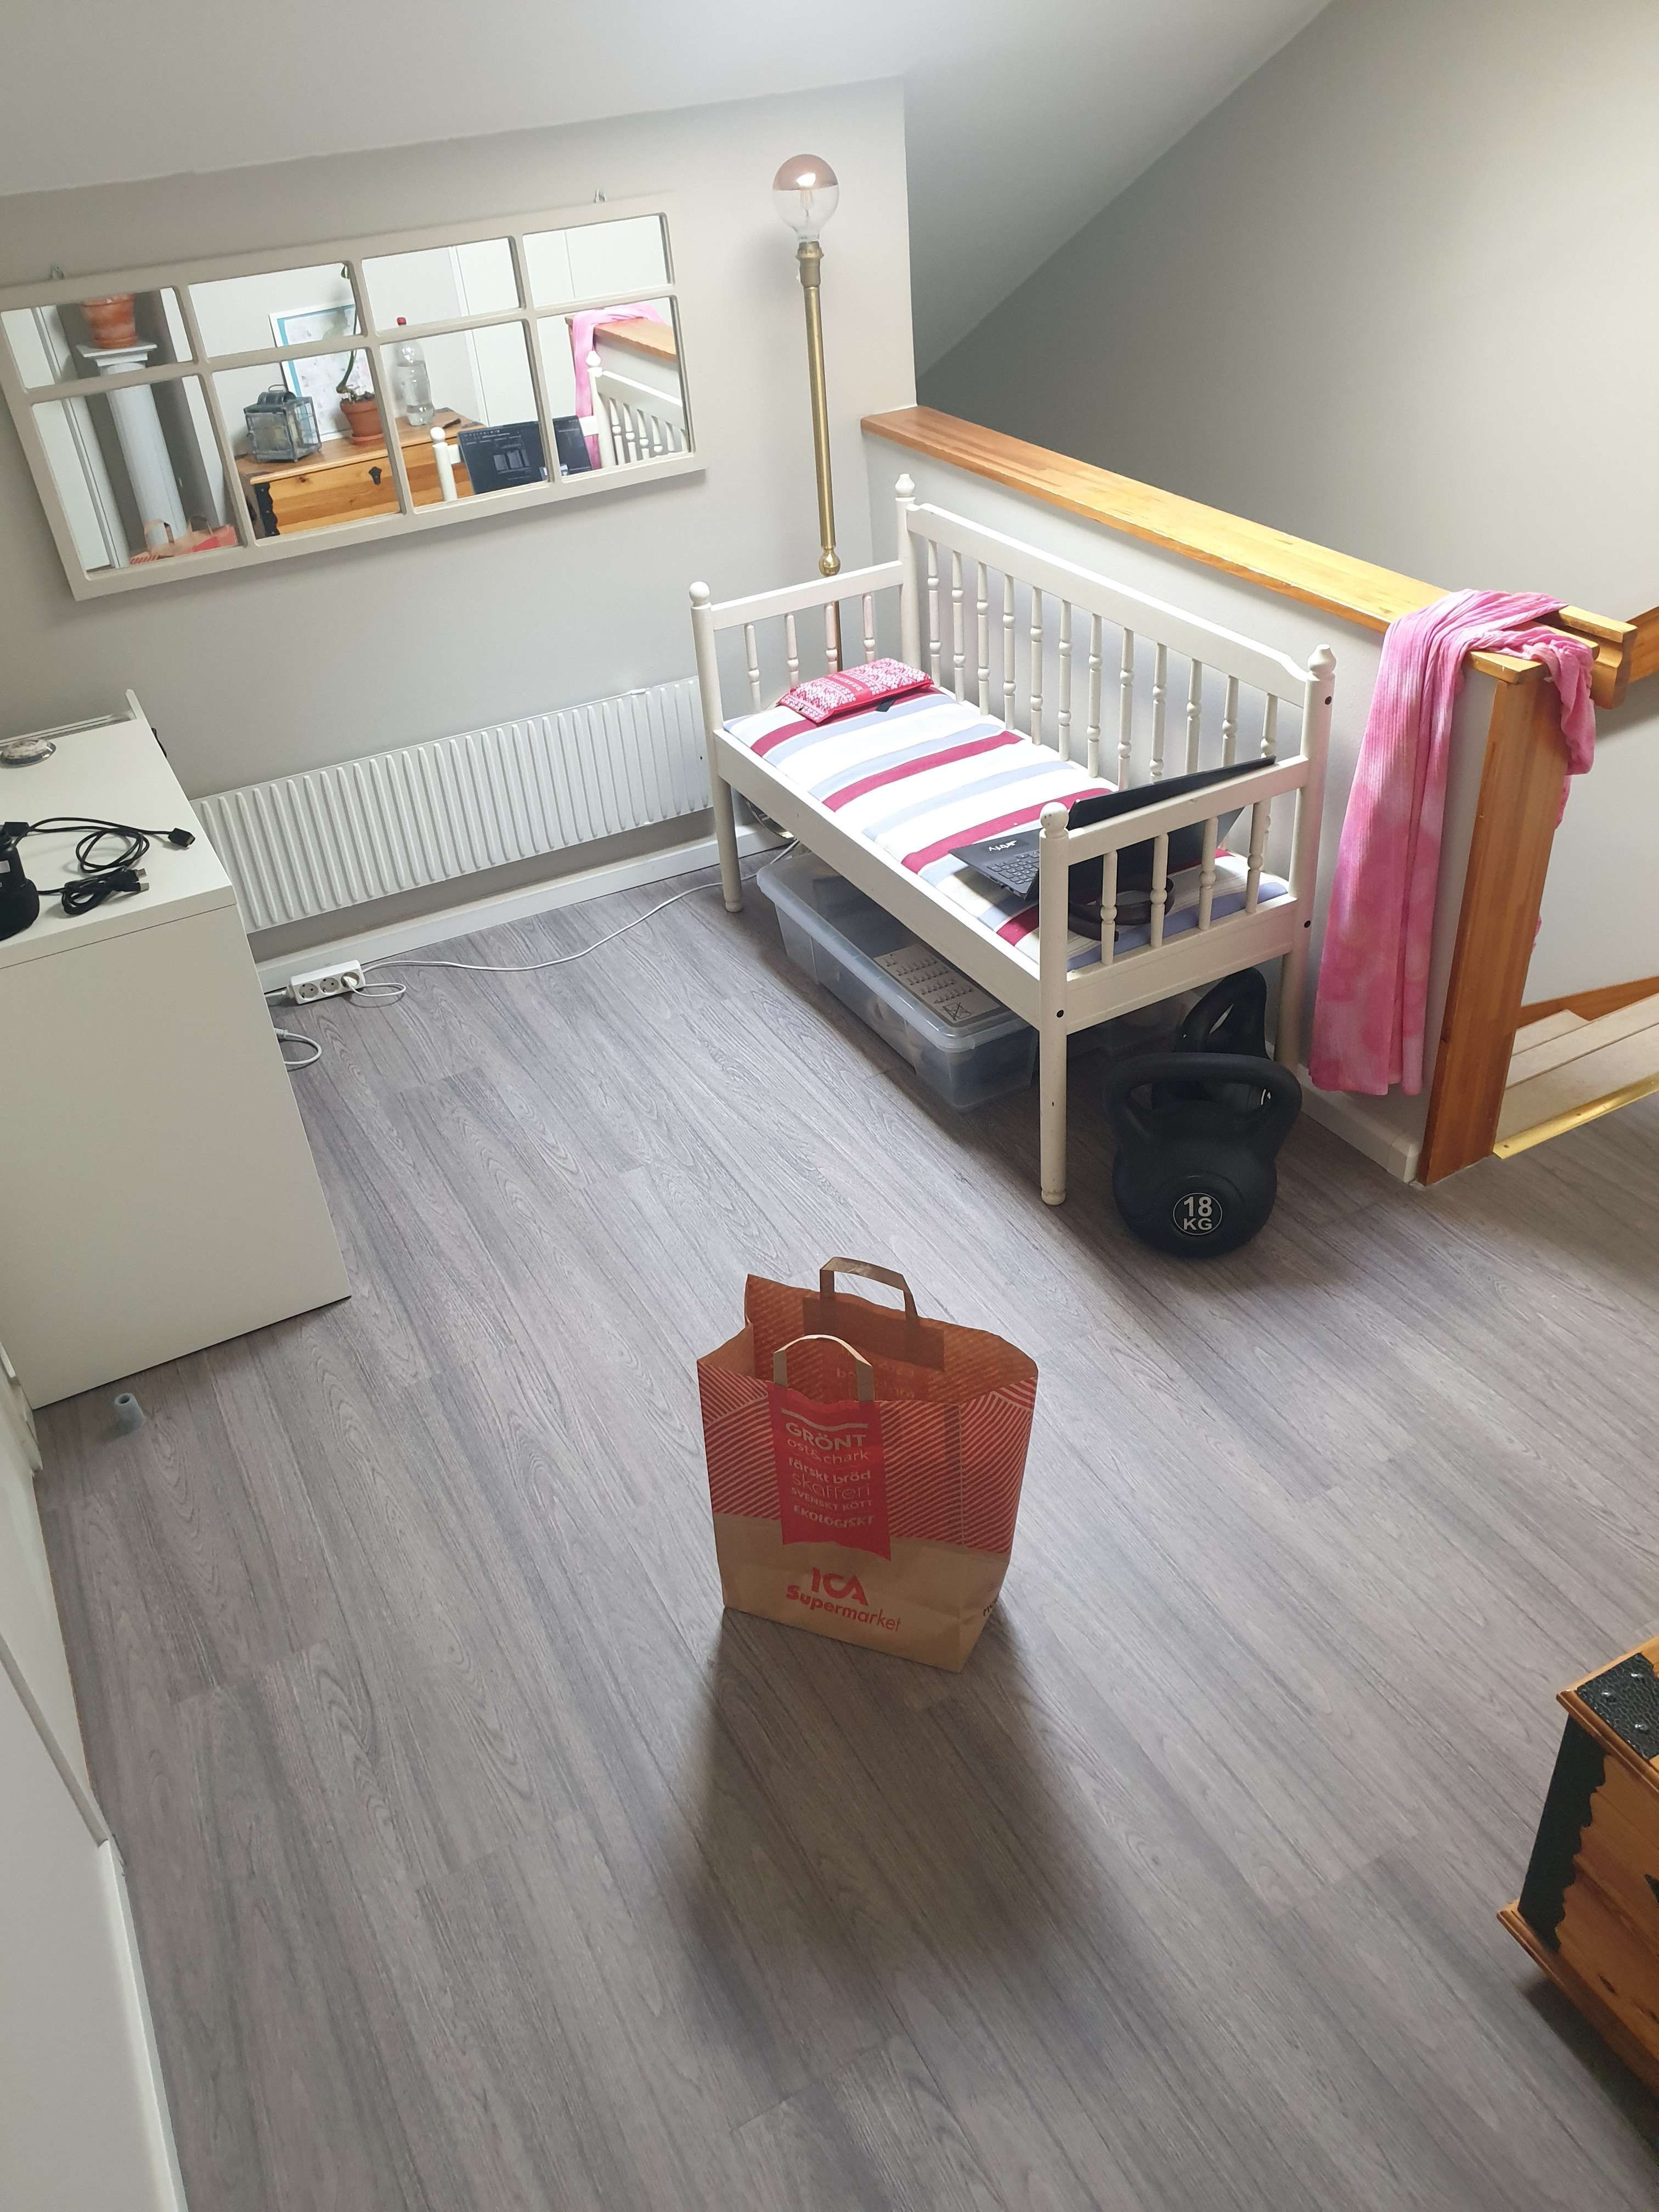
\includegraphics[width=\columnwidth]{images/real_world_map.jpg}
    \caption{Real-world test environment.}
    \label{fig:real_world_map}
\end{figure}

%------------------------------------------------------------------------------------------


%------------------------------------------------------------------------------------------
\begin{comment}
    Italicize symbols ($T$ might refer to temperature, but T is the unit tesla).

    Refer to ``\eqref{eq},'' not ``Eq. \eqref{eq}''
    
    It is good practice to explain the significance of the figure in the caption.
    
    Figure axis labels are often a source of confusion. Use words rather than symbols. As an example, write the quantity ``Magnetization,'' or ``Magnetization M,'' not just ``M.'' Put units in parentheses. Do not label axes only with units. As in Fig. 1, for example, write ``Magnetization (A/m)'' or ``Magnetization (A$\cdot$m$^{-1}$),'' not just ``A/m.'' Do not label axes with a ratio of quantities and units. For example, write ``Temperature (K),'' not ``Temperature/K.''
    
    When referencing your figures and tables within your paper, use the abbreviation ``Fig.'' even at the beginning of a sentence. Do not abbreviate ``Table.'' Tables should be numbered with Roman Numerals.
      
    In this section, the method used to find an answer to the research questions should be presented.
    
    If this report presents results from a literature search, this means providing sufficient information for allowing someone else to repeat the literature search and compare the results. I.e., a search using the phrases a, b, and c, was made in database x, y and z on the date Month Date, Year (e.g., July 31st, 2021). The search resulted in x hits. Then, information on how you chose which works to include in this report should be provided. The references should be used for answering your research questions.
    
    If the work reports on an experiment, this part should provide information about the experimental setup, how the experiment was conducted, how data was collected and analyzed etc. Motivate methodological choices through references. Also an experiment should be presented with sufficient detail such that it can be repeated by someone else.
\end{comment}
%------------------------------------------------------------------------------------------
\section{Results}
\label{section:results}
%------------------------------------------------------------------------------------------
% Simulation

% Map
The SLAM map obtained during simulation is shown in Fig.\:\ref{fig:simulation_slam_map}.
\begin{figure}
    \centering
    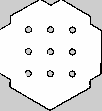
\includegraphics[width=\columnwidth]{images/simulation_SLAM_map.png}
    \caption{Map generated using SLAM in simulation.}
    \label{fig:simulation_slam_map}
\end{figure}
% Evaluation metrics
The performance of the simulated system in terms of the evaluation metrics has been summarized in Table.\:\ref{tab:simulation_metrics}.
\begin{table}
    \centering
    \resizebox{\columnwidth}{!}{\noindent\begin{tabular}{|c|c|} \hline
         \textbf{Number of collisions}  & \textbf{Processing time per sensor update (ms)}       \\ \hline
         $0$                            & Could not be measured                                 \\ \hline
    \end{tabular}}
    \caption{Evaluation metrics obtained during testing of the simulated system.}
    \label{tab:simulation_metrics}
\end{table}

%------------------------------------------------------------------------------------------
% Real world

% Map
The map obtained using SLAM during real-world deployment can be seen in Fig.\:\ref{fig:real_world_slam_map}.
\begin{figure}
    \centering
    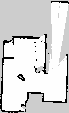
\includegraphics[width=\columnwidth]{images/real_world_SLAM_map.png}
    \caption{SLAM map obtained during real-world deployment of the developed system.}
    \label{fig:real_world_slam_map}
\end{figure}
% Evaluation metrics
The systems performance in real-world deployment is shown in Table\:\ref{tab:real_world_metrics}.
\begin{table}
    \centering
    \resizebox{\columnwidth}{!}{\noindent\begin{tabular}{|c|c|c|} \hline
         \textbf{Number of collisions}  & \textbf{Processing time per sensor update (ms)}       \\ \hline
         $0$                            & Could not be measured                                 \\ \hline
    \end{tabular}}
    \caption{Evaluation metrics obtained during real-world deployment and testing of the system.}
    \label{tab:real_world_metrics}
\end{table}


%------------------------------------------------------------------------------------------


%------------------------------------------------------------------------------------------
\begin{comment}
    
\end{comment}
%------------------------------------------------------------------------------------------
\section{Discussion}
%------------------------------------------------------------------------------------------
% Results

%======================================================
% SLAM map

% SLAM maps obtained from both simulation and real-world
The resulting maps obtained during simulation and real-world testing using SLAM (see Fig.\:\ref{fig:simulation_slam_map} and Fig.\:\ref{fig:real_world_slam_map}) were close to identical to the ground truth maps (see Fig.\:\ref{fig:simulation_map} and Fig.\:\ref{fig:real_world_map}), with only minor inconsistencies and slight skew. Thus providing very promising results in terms of mapping capabilities in small and simple environments.
% Stairs
It is worth noting that since a 2D LIDAR was used, the stairs in the real-world testing environment (see Fig.\:\ref{fig:real_world_map}) just gets mapped as free space (see Fig.\:\ref{fig:real_world_slam_map}).

%======================================================
% Evaluation metrics

% Collisions
The number of collisions in both simulation and real-world deployment can be explained by the quality of the SLAM maps. Since the testing environments were static, only static obstacles are a threat (dynamic obstacles are not present). Hence because the SLAM algorithm was able to achieve and provide very accurate maps, the algorithm was able to localize itself very well and easily avoid static obstacles.

% Processing time per sensor update
% 4th criteria
Implementing code to measure the processing time per sensor update could not be finished because of time constraints. The project thus failed to report on the second evaluation metric (simulation and real-world) and to evaluate the fourth criteria. The fourth criteria (see Introduction\:\ref{section:intro}) is thus considered not achieved.
% Improve performance
However, the metric and criteria remained included (despite the inability to measure it) because the authors feel that the metric and criteria are essential to accurately evaluate the system and identify potential limitations. A few potential computational improvements are therefor outlined to help guide future work to better meet the fourth criteria.
% Composition nodes + IPC
First, the use of composition nodes in ROS2 has shown a substantial increase in performance and marks a possibly substantial improvement to the computation (CPU usage), memory and latency of the system, especially if combined with intra-process communication (IPC)\:\cite{macenski_impact_2023}.
% Subset of LIDAR points
Secondly, when using LIDAR for SLAM, one can consider using only a subset of all the LIDAR points, therefor reducing computational load, but trading it for a reduction in information\:\cite{filip_lidar_2023}.

\begin{comment}
% 5th criteria
As seen in the Results\:\ref{section:results}, the system achieved consistent SLAM maps during testing scenarios lasting over one hour. The fifth criteria (see Introduction\:\ref{section:intro}) was therefor fulfilled by the system. This indicates that the algorithms have sufficient performance for longer sessions (as is supported by research for SLAM Toolbox\:\cite{macenski_slam_2021} and Navigation2\:\cite{macenski_marathon_2020}). Additionally, the robot design, in terms of storage (for the map) and energy storage, proved sufficient for longer mapping sessions.
\end{comment}

%======================================================
% Test environments/scenarios

% Things not considered/tested
The system was not assessed in scenarios with different temperatures, light conditions, surfaces (e.g. uneven and different types), weather conditions like rain and fog, humidity and moisture, electromagnetic interference (EMI), and dynamic environments. Additionally, the impact of artificial versus natural light was not compared.
% Implication and why they were not tested
The system was designed to be able to handle some of these conditions (see the criteria in Introduction\:\ref{section:intro}), but sufficient resources could not be allocated to test the system in all necessary conditions. It is important that the system is evaluated in all the listed scenarios in future work to accurately establish the limitations of the system.
% 1st criteria
This makes evaluation of the first criteria from the Introduction\:\ref{section:intro} unresolved and is therefor considered not satisfied.

%------------------------------------------------------------------------------------------
% Problems

%======================================================
% Robot design

% Thresholds, cables, carpets
Given the design of the robot and the size of the wheels (mainly the small spherical wheels), obstacles such as thresholds, carpets and cables proved problematic for the robot to traverse. 
% 4 wheel limitations
The four wheel design also poses stability issues in uneven terrain where driving wheels might loose contact with the ground, damaging the performance of the robot and possibly resulting in the robot getting stuck. 
% 2nd criteria
These scenarios are common in human-made environments leading to the developed system failing to meet the second criteria established in the Introduction\:\ref{section:intro}.
% Future design
Future design would use only one stabilizing wheel, a caster wheel, and altering the location of the motorized wheels, thus moving to a three wheel design. This would improving stability and help the robot more easily scale carpet edges, cables lying on the floor, thresholds and similar. 

%======================================================
% Sensors

% Fusion
Sensor noise and other environmental factors like lighting variations (e.g. return signal overwhelmed by sunlight), sensor beams being reflected of environmental particles like rain and dust, all pose serious problems for SLAM\:\cite{corke_robotics_2023}. However, temporal fusion and sensor fusion can help mitigate these problems\:\cite{siegwart_introduction_2011}.
% Sensor fusion
Sensor fusion was employed in this project, but an additional sensor for measuring the surrounding could have helped to further improve performance by negating the limitations of the LIDAR. A good candidate would be a camera since it would complement the features offered by a LIDAR well (see Introduction\:\ref{section:intro})\:\cite{chen_slam_2022}. It is important to note that this would increase the computational complexity and future work needs to investigate this further\:\cite{chen_slam_2022}. 
% Temporal fusion
Temporal fusion also deserves consideration in future work. It could not be found that any of the toolboxes used in this project made use of temporal fusion.

% LIDAR -> RADAR
While this project used a LIDAR, expansion to dynamic environments should consider the use of a RADAR instead of a LIDAR since it can measure speed of objects\:\cite{ilas_electronic_2013}, which could help with collision avoidance. Additionally, a RADAR might offer better performance in low visibility weather conditions and harsh environments, like environments containing significant amount of dust particles\:\cite{fritsche_fusing_2018}.

% LIDAR limitations
% Reflection
A potential issue for some range sensors is that they can have their entire signal absorbed or coherently reflected (no reflection is received by the sensor) such that the sensor output is NaN or the maximum possible value\:\cite{siegwart_introduction_2011}\cite{corke_robotics_2023}.
% Sensor aliasing
Another problem is sensor aliasing (also known as perceptual aliasing\:\cite{cadena_past_2016}), which is the difficulty for the robot to distinguish between states because it is given non unique data\:\cite{siegwart_introduction_2011}. This is the case for environments which are sparse, geometrically repetitive, and if the environment lacks sufficient amount of distinct features\:\cite{cai_lidarinertial_2023}.
The problem stems from sensory inputs and states seeming identical to the robot\:\cite{siegwart_introduction_2011}. In all of these scenarios, the sensor values either remains unchanged, is not unique or there is insufficient amount of data\:\cite{cai_lidarinertial_2023}\cite{siegwart_introduction_2011}.
A simple example which illustrates this is a robot only equipped with range-based sensors, for this robot, all hallways with equal distance between the walls seem identical. 
% Empty
It is also possible that there are no objects within sensor range, complicating localization and mapping since the robot is unable to observe anything in its surrounding\:\cite{siegwart_introduction_2011}\cite{corke_robotics_2023}.
% Rotating part
Moreover, since LIDARs have a rotating part\:\cite{ilas_electronic_2013} there is a small delay between all the LIDAR beam and value pairs. Hence the array of values provided by the LIDAR are not all from the exact same time instant, and therefor does not correspond to the exact same robot position (if the robot is moving).
% Loop closure
Additionally, LIDARs can struggle with loop closure because of its difficulty in extracting features (see Introduction\:\ref{section:intro})\:\cite{khan_investigation_2022}.
% How this affects the system
All of these issues signify limitations of using only a LIDAR as the sole sensor for measuring the surrounding, as was done in this project.
% 3rd criteria
The system does however fulfill the third criteria (see Introduction\:\ref{section:intro}) because of the chosen sensors, namely a LIDAR with sufficient range.

%======================================================
% Errors and drift

% Robot mass and slip
The constructed robot had significant wheel slip because of low mass and thus poor traction, which results in a substantial source of errors.
% Drift
Given the duality introduced in the Introduction\:\ref{section:intro}, an error in pose estimation or the map can be critical since this error will grow and errors will accumulate, further degrading the map and pose estimation\:\cite{siegwart_introduction_2011}\cite{zhao_occupancy-slam_2022}. A common source of this error is actuator noise which includes: floor contact (e.g. wheel slip, wheel deformation, uneven floor) and poor resolution of values (e.g. time, sensor measurements)\:\cite{siegwart_introduction_2011}\cite{corke_robotics_2023}. All of this can contribute to erroneous integration which leads to error accumulation which will grow with time which leads to further errors in position estimate and map drift\:\cite{siegwart_introduction_2011}\cite{corke_robotics_2023}.

\begin{comment}
% Correlation
Sensor errors will always be present and the SLAM algorithm is always going to make some mistakes. Thus the spatial correlation of map features introduced in the Introduction\:\ref{section:intro} will never achieve full correlation. This in turn will limit the awareness of the algorithm and its ability to make intelligent decisions, confining it to some degree to local information. The reason being that if full correlation is not achieved, then information of an object or feature (could also be the robot itself), does not necessarily allow the algorithm to determine how it relates to a second object, despite having seen both previously in this scenario. The algorithm can not use correlation information to figure this out because the correlation is not complete because of sensor errors and mistakes. Thus forcing the algorithm to rely on local sensor information, hurting its awareness and limiting its ability to make intelligent decisions. One can imagine the results of this being as if the map only contains disconnected fragments, and the robot being confined only to its current fragment, unable to see or make use of the entirety of the map. It is important to not mistakenly interpret that this concerns the absolute position of features on the map, this only concerns how features relate to each other, not their absolute position.
\end{comment}

%======================================================
% SLAM limitations

% Dynamic environments
SLAM still has a number of weak points, including limited capabilities in dynamic environments (since most SLAM algorithms assume static environments)\:\cite{siegwart_introduction_2011}\cite{sousa_systematic_2022}, as well as harsh environments\:\cite{cadena_past_2016}. 
% SLAM parameters
Additionally, the parameters for most SLAM algorithms are specific to the environment where their task is defined, thus complicating their deployment in different environments\:\cite{khole_comprehensive_2023}.
% Data association
SLAM is also sensitive to incorrect data association (incorrect matching of features), particularly during loop closure\:\cite{siegwart_introduction_2011}, and sensor aliasing complicates this even further\:\cite{cadena_past_2016}. 
% Loop closing
Erroneous loop closing is similarly inevitable in the presence of sensor aliasing, causing significant damage to the SLAM results\:\cite{cadena_past_2016}.
% More info
This report is unable to cover all SLAM limitations and problems. The interested reader is hence refereed to the comprehensive survey by Cadena \textit{et al.}\:\cite{cadena_past_2016}, which extensively covers the limitations, difficulties and open problems present in SLAM research (including sensor failures, outliers, solvers failing to converge to global minimum, and unbounded growth in memory and computation). For specific focus on the limitations present in long-term deployment of SLAM, see the thorough literature review by Sousa \textit{et al.}\:\cite{sousa_systematic_2022}.
% Implication
It is important to consider these problems since they limit the robot, despite the advanced SLAM algorithms currently available.

%======================================================
% Navigation limitations

% DWB
While DWB (default local trajectory tracker of Navigation2) is very flexible and configurable, it does suffer from interrelated parameters which can damage performance if not tuned correctly, which is complex and not a trivial task\:\cite{macenski_desks_2023}.

%======================================================
% Future

It is the main goal in future work to make the robot completely autonomous (removing the need for users to issue waypoints) and for all code to run on the robot without the use of an external PC.

%------------------------------------------------------------------------------------------


%------------------------------------------------------------------------------------------
\begin{comment}
    % Kidnapped robot
    %Another limitation common in SLAM algorithms is the kidnapped robot problem\:\cite{siegwart_introduction_2011}. The reason being that most algorithms struggle with localization if the robot has been moved, most algorithms continue to believe that the robot still is somewhere at the old location, failing to realize it has been moved\:\cite{siegwart_introduction_2011}.

    % Nav2 overkill
    %The advanced algorithms used by Navigation2 far exceeds what is required for the simple circular differential drive robot used in this project, and a simple A* algorithm would have sufficed\:\cite{macenski_open-source_2024}.
    
    %With Kalman filter localization, even bad measurements improve the certainty of the estimate of the robots position\:\cite{siegwart_introduction_2011}.
\end{comment}
%------------------------------------------------------------------------------------------

\section{Conclusion}
%------------------------------------------------------------------------------------------

The system met one out of the four criteria established and failed to evaluate one of the evaluation metrics. However, it did achieve favorable SLAM results in small environments, hence warranting further development to revise the shortcomings of the system. The results show that the software, in terms of the toolboxes used, proved capable for the task, thus showing that the robot design was the limiting factor.

%------------------------------------------------------------------------------------------


%------------------------------------------------------------------------------------------
\begin{comment}
    
\end{comment}
%------------------------------------------------------------------------------------------
% Appendix should be before ackowledgment
%\section*{Appendix}
%------------------------------------------------------------------------------------------



%------------------------------------------------------------------------------------------


%------------------------------------------------------------------------------------------
\begin{comment}
    Appear before acknowledgment
\end{comment}
%------------------------------------------------------------------------------------------
%\section*{Acknowledgment}
%------------------------------------------------------------------------------------------



%------------------------------------------------------------------------------------------


%------------------------------------------------------------------------------------------
\begin{comment}
    
\end{comment}
%------------------------------------------------------------------------------------------

%------------------------------------------------------------------------------------------
% Select the IEEEtran style
\bibliographystyle{IEEEtran}
% Include bibliography file
\bibliography{refs, ELA408}
%------------------------------------------------------------------------------------------

\end{document}